\documentclass[10pt, a4paper, italian]{article}
\usepackage[T1]{fontenc}
\usepackage[utf8]{inputenc}
\usepackage{amsmath, amssymb, amsthm, thmtools, amsfonts, mathtools}
\usepackage{nicefrac}
\usepackage{calc}
\usepackage[pdftex, hyperindex, plainpages=false]{hyperref}
\usepackage[nameinlink]{cleveref} %load before classicthesis (clash)
%\usepackage[nochapters,pdfspacing]{classicthesis}
\usepackage{siunitx}
\usepackage[siunitx]{circuitikz}

\usepackage[a4paper]{geometry}
\usepackage{float}
\usepackage{mdframed}
\usepackage{titling}
\usepackage{booktabs}
\usepackage{graphicx}
\usepackage{caption, subcaption}
\usepackage{xcolor}
\usepackage[italian]{babel}
\usepackage{pgfplots}
\usepackage{listings}
%\usepackage{lmodern}
\usepackage{url}
\usepackage{enumitem}
\usepackage{tikz} %loads after classicthesis (xcolor incompat)

% lets graphicx know path where figures to be included are found
\graphicspath{{../figs/}}
\makeatletter
\def\input@path{{../figs/}}
%or: \def\input@path{{/path/to/folder/}{/path/to/other/folder/}}
\makeatother

% tikz pgf plots setup
\usepgfplotslibrary{external}
\pgfplotsset{compat=1.15}
%\tikzexternalize

% spaces and significant digits/figures for measurements
\sisetup{free-standing-units, space-before-unit, number-unit-product = \;,
scientific-notation = false, round-mode = figures, round-precision = 1,}

% turns all (hyperlinked) references black [default is blue]
\hypersetup{
	linktoc=all,
	colorlinks=true,
	linkcolor=black
}

% code listings config
%\lstset{
%language=Python,
%basicstyle=\ttfamily,
%columns=fullflexible,
%keepspaces=true,
%}

% mdframed (for boxed text) configuration
\mdfsetup{linewidth=0.6pt}

% Default fixed font does not support bold face
\DeclareFixedFont{\ttb}{T1}{txtt}{bx}{n}{12} % for bold
\DeclareFixedFont{\ttm}{T1}{txtt}{m}{n}{12}  % for normal

% Custom colors
\usepackage{color}
\definecolor{deepblue}{rgb}{0,0,0.5}
\definecolor{deepred}{rgb}{0.6,0,0}
\definecolor{deepgreen}{rgb}{0,0.5,0}

% Commands 
\newcommand{\executeiffilenewer}[3]{%
	\ifnum\pdfstrcmp{\pdffilemoddate{#1}}%
		{\pdffilemoddate{#2}}>0%
	{\immediate\write18{#3}}\fi%
}
% input .svg --> .pdf_tex graphs
%\newcommand{\includesvg}[1]{%
%	\executeiffilenewer{#1.svg}{#1.pdf}%
%	{inkscape -z -D --file=#1.svg %
%	--export-pdf=#1.pdf --export-latex}%
%	\input{#1.pdf_tex}%
%}
% Thanks UniPi's Department of Physics E. Fermi
\newcommand{\thanksdf}{(\thanks{Dipartimento di Fisica E.~Fermi,%
Universit\`a di Pisa - Pisa, Italy.}\;)}

% hyperlink to email address
\newcommand{\mail}[1]{\href{mailto:#1}{\textsf{#1}}}

% \vec for bold vectors, instead of overarrows (now "\arrvec")
\let\arrvec=\vec
\renewcommand{\vec}[1]{\boldsymbol #1}
% replaces straight phi with slanted phi
\renewcommand{\phi}{\varphi}
% replaces straight eps with curved epsilon
\newcommand{\eps}{\varepsilon}
% abbreviation for (sub_/super^)scripts of \lim, \sum,... in inline math
\newcommand{\ds}{\displaystyle}

% blackboard/number set letters
\newcommand{\CC}{\mathbb C}
\newcommand{\HH}{\mathbb H}
\newcommand{\KK}{\mathbb K}
\newcommand{\NN}{\mathbb N}
\newcommand{\PP}{\mathbb P}
\newcommand{\QQ}{\mathbb Q}
\newcommand{\RR}{\mathbb R}
\newcommand{\ZZ}{\mathbb Z}

\newcommand{\Abs}[1]{{\left\Vert #1\right\Vert}}
\newcommand{\enclose}[1]{{\left( #1 \right)}}
\newcommand{\Enclose}[1]{{\left[ #1 \right]}}
\newcommand{\floor}[1]{\left\lfloor #1 \right\rfloor}
\newcommand{\ceil}[1]{\left\lceil #1 \right\rceil}
\newcommand{\To}{\rightrightarrows}

% Math operators
\DeclareMathOperator{\divergence}{div}
\renewcommand{\div}{\divergence}
\DeclareMathOperator{\Imaginarypart}{Im}
\renewcommand{\Im}{\Imaginarypart}
\DeclareMathOperator{\Realpart}{Re}
\renewcommand{\Re}{\Realpart}
%\DeclareMathOperator{\arg}{arg}
\DeclareMathOperator{\tg}{tg}
\DeclareMathOperator{\arctg}{arctg}
\DeclareMathOperator{\settsinh}{settsinh}
\DeclareMathOperator{\settcosh}{settcosh}
\DeclareMathOperator{\tr}{tr}
\DeclareMathOperator{\im}{im}
\DeclareMathOperator{\sgn}{sgn}
\DeclareMathOperator{\diag}{diag}

\DeclarePairedDelimiter{\norm}{\lVert}{\rVert}
\DeclarePairedDelimiter{\scalar}{\langle}{\rangle}

% Logarithm with arbitrary base.
% -> log_10
\newcommand{\llog}[1][10]{\log_{#1}}

% Absolute value.
% -> |x|
\newcommand{\abs}[1]{\left| #1 \right|}

% Powers.
% -> x^a
\newcommand{\power}[2][2]{\left( #2 \right)^{#1}}

% Square.
% -> x^2
\newcommand{\sq}[1]{\power[2]{#1}}

% Expansion of the binomial coefficient.
% -> n1!/(n2!(n1 - n2)!)
\newcommand{\binomexpr}[2]{\frac{#1!}{#2!(#1 - #2)!}}

% Expression evaluation at a given point with square brackets.
% -> [x]_{a}
\newcommand{\at}[2]{\left[ #1\right]_{\makebox[-1pt][l]{${\scriptstyle#2}$}}}

% Expression evaluation in an interval.
% -> [x] _{a}^{b}
\newcommand{\eval}[3]{\left.#1%
  \right|_{\makebox[-1pt][l]{${\scriptstyle#2}$}}^{\makebox[-1pt][l]{${\scriptstyle#3}$}}}

% Upright d in math mode (for differentials).
% -> d
\newcommand{\ud}{\mathrm{d}}

% Differential.
% -> dx
\newcommand{\diff}[1][x]{\,\ud{#1}}

% Base command for defining derivatives.
% -> df/dx or d^kf/dx^k
\newcommand{\basederivative}[4][]{%
  \displaystyle%
  \ifx\\#1\\\frac{#4#2}{#4#3}%
  \else%
  \frac{#4^#1#2}{#4#3^#1}%
  \fi%
}

% Total derivative.
% -> df/dx(x) or d^kf/dx^k(x)
\newcommand{\td}[4][]{%
  \basederivative[#1]{#2}{#3}{\ud}%
  \ifx\\#4\\%
  \else%
  \mkern-4mu\left(#4\right)%
  \fi%
}

% Partial derivative.
% -> df/dx(x) or d^kf/dx^k(x)
\newcommand{\pd}[4][]{%
  \basederivative[#1]{#2}{#3}{\partial}%
  \ifx\\#4\\%
  \else%
  \mkern-4mu\left(#4\right)%
  \fi%
}

\newcommand{\intinf}{\int_{-\infty}^{\infty}\!\!\!}

\newcommand{\cinterval}[2]{\left[\, #1,~#2 \,\right]}

\newcommand{\linterval}[2]{\left[\, #1,~#2 \,\right)}

\newcommand{\rinterval}[2]{\left(\, #1,~#2 \,\right]}

\newcommand{\ointerval}[2]{\left(\, #1,~#2 \,\right)}

\newcommand{\prob}[1]{\displaystyle P\left(#1\right)}

\newcommand{\pvalue}{\emph{$p$-value}}

\newcommand{\cond}{\,|\,}

\newcommand{\expect}[1]{\displaystyle E\left[#1\right]}

\newcommand{\mom}[2][]{\displaystyle {\cal M}_{#2}\ifx\\#1\\\else(#1)\fi}

\newcommand{\momalg}[1]{\displaystyle \lambda_{#1}}

\newcommand{\momcen}[1]{\displaystyle \mu_{#1}}

\newcommand{\skewness}{\displaystyle \gamma_1}

\newcommand{\kurtosis}{\displaystyle \gamma_2}

\newcommand{\charf}[1][x]{\phi_{#1}}

\newcommand{\momgenf}[1][x]{M_{#1}}

\newcommand{\fwhm}{{\scriptstyle \textsc{FWHM}}}

\newcommand{\hwhm}{{\scriptstyle \textsc{HWHM}}}

\newcommand{\median}{\mu_{\nicefrac{1}{2}}}

\newcommand{\var}[1]{\ensuremath{\text{Var}\left(#1\right)}}

\newcommand{\cov}[2]{\ensuremath{\text{Cov}\left(#1, #2\right)}}

\newcommand{\corr}[2]{\ensuremath{\text{Corr}\left(#1, #2\right)}}

\newcommand{\like}{\mathcal L}

\newcommand{\likelihood}[2][]{\like\ifx\\#2\\\else(#2\ifx\\#1\\\else;#1\fi)\fi}

\newcommand{\chisq}{\ensuremath{\chi^2}}

\newcommand{\chisquare}[2][]{\chisq\ifx\\#2\\\else(#2\ifx\\#1\\\else;#1\fi)\fi}

\newcommand{\loglikelihood}[2][]{\log\likelihood[#1]{#2}}

\newcommand{\pdf}[3][]{#2(#3\ifx\\#1\\\else;#1\fi)}

\newcommand{\binomialpdf}[2][]{\pdf[#1]{\mathcal B}{#2}}

\newcommand{\multinomialpdf}[2][]{\pdf[#1]{\mathcal M}{#2}}

\newcommand{\poissonpdf}[2][]{\pdf[#1]{\mathcal P}{#2}}

\newcommand{\uniformpdf}[2][]{\pdf[#1]{u}{#2}}

\newcommand{\exponentialpdf}[2][]{\pdf[#1]{\varepsilon}{#2}}

\newcommand{\gausspdf}[2][]{\pdf[#1]{N}{#2}}

\newcommand{\chisquarepdf}[2][]{\pdf[#1]{\wp}{#2}}

\newcommand{\cauchypdf}[2][]{\pdf[#1]{c}{#2}}

\newcommand{\erf}[1]{\ensuremath{\text{erf}\left(#1\right)}}

\newcommand{\dccases}[4][]{#2 \ifx\\#2\\\else=\fi %
  \begin{cases}
    \displaystyle #3 & \text{per variabili discrete}\\
    \displaystyle #4 & \text{per variabili continue}#1
  \end{cases}
}
% sub/super-scriptable for all symbol as math operator 
\newcommand\Scaleforall[1]{\vcenter{\hbox{\scalefont{#1}$\forall$}}}

\DeclareMathOperator*\forevery{%
  \vphantom\sum
  \mathchoice{\Scaleforall{2}}{\Scaleforall{1.4}}{\Scaleforall{1}}{\Scaleforall{0.75}}}
\usepackage{multicol}
\geometry{left=2cm, right=2cm, top=2cm, bottom=2cm}

% indexes subsections with letters, sections with numbers (1.a, 1.b, ...)
\renewcommand{\thesubsection}{\thesection.\alph{subsection}}

% lets graphicx know path where figures to be included are found
\graphicspath{{../figs/}}

\author{Gruppo 1.AC \\ Matteo Rossi, Bernardo Tomelleri}
\title{EsD4 ADC-DAC: Convertitore sigma-delta}
\begin{document}
\date{\today}
\maketitle

\section*{Misura componenti dei circuiti}
\begin{table}[htbp]
\centering
\begin{tabular}{cccccc}
\toprule
Resistenze $[\si{\ohm}]$ & $R$ & $\sigma R$ & Capacità $[\si{n\F}]$ & $C$ &
$\sigma C$ \\
\midrule
\midrule
$R_1$	  	& 992 	& 8		& $C_1$ & 99	& 4 \\
$R_2$	  	& 994	& 8		& & & \\
$R_3$	  	& 993	& 8		& & & \\
$R_4$	  	& 994 	& 8	& & & \\
$R_5$	  	& 996	& 8 & & & \\
\bottomrule   
\end{tabular}
\caption{Valori di resistenza e capacità misurate con il multimetro dei
componenti del primo circuito.}

\begin{tabular}{cccccc}
\toprule
Resistenze $[\si{\ohm}]$ & $R$ & $\sigma R$ & Capacità $[\si{n\F}]$ & $C$ &
$\sigma C$ \\
\midrule
\midrule
$R_1$	  	& 995 	& 8		& $C_1$ & 109	& 4 \\
$R_2$	  	& 999	& 8		& & & \\
$R_3$	  	& 998	& 8		& & & \\
$R_4$	  	& 998 	& 8	& & & \\
$R_5$	  	& 996	& 8 & & & \\
\bottomrule   
\end{tabular}
\caption{Valori di resistenza e capacità misurate con il multimetro
dei componenti del secondo circuito}
\end{table}

Riportiamo per completezza anche i valori delle tensioni di alimentazione
continue per i circuiti integrati misurate con il multimetro
\begin{align*}
V_{CC} &= 4.99 \pm 0.03 \; \si{\V} \\
V_{EE} &= -4.99 \pm 0.03 \; \si{\V}
\end{align*}

Per tutto il resto della trattazione come ampiezze dei segnali si intendono
misurate non ``picco - picco'', a meno che non venga esplicitato altrimenti.

\setcounter{section}{0}
%=======================
\section{Analisi e costruzione del circuito}\label{sec: AC}
\subsection{Costruzione del circuito}
Si è costruito il circuito secondo lo schema riportato in \cref{schm: ADC},
alimentando con $V_{CC} = 5 \; \si{\V}$ il D Flip-Flop e gli OpAmp alla
medesima $V_{CC}$ e $V_{EE} = -5 \; \si{\V}$ con l'AD2.
Dunque abbiamo collegato l'ingresso analogico \verb+V3+ del circuito al
canale 1 del Waveforms (generator) e il pin CLK del FF ad un segnale di
clock di frequenza $f\ped{clk} = 50 \; \si{k\Hz}$ generato in DIO 0 con
Patterns (generator).
\begin{figure}[htbp]
    \centering
	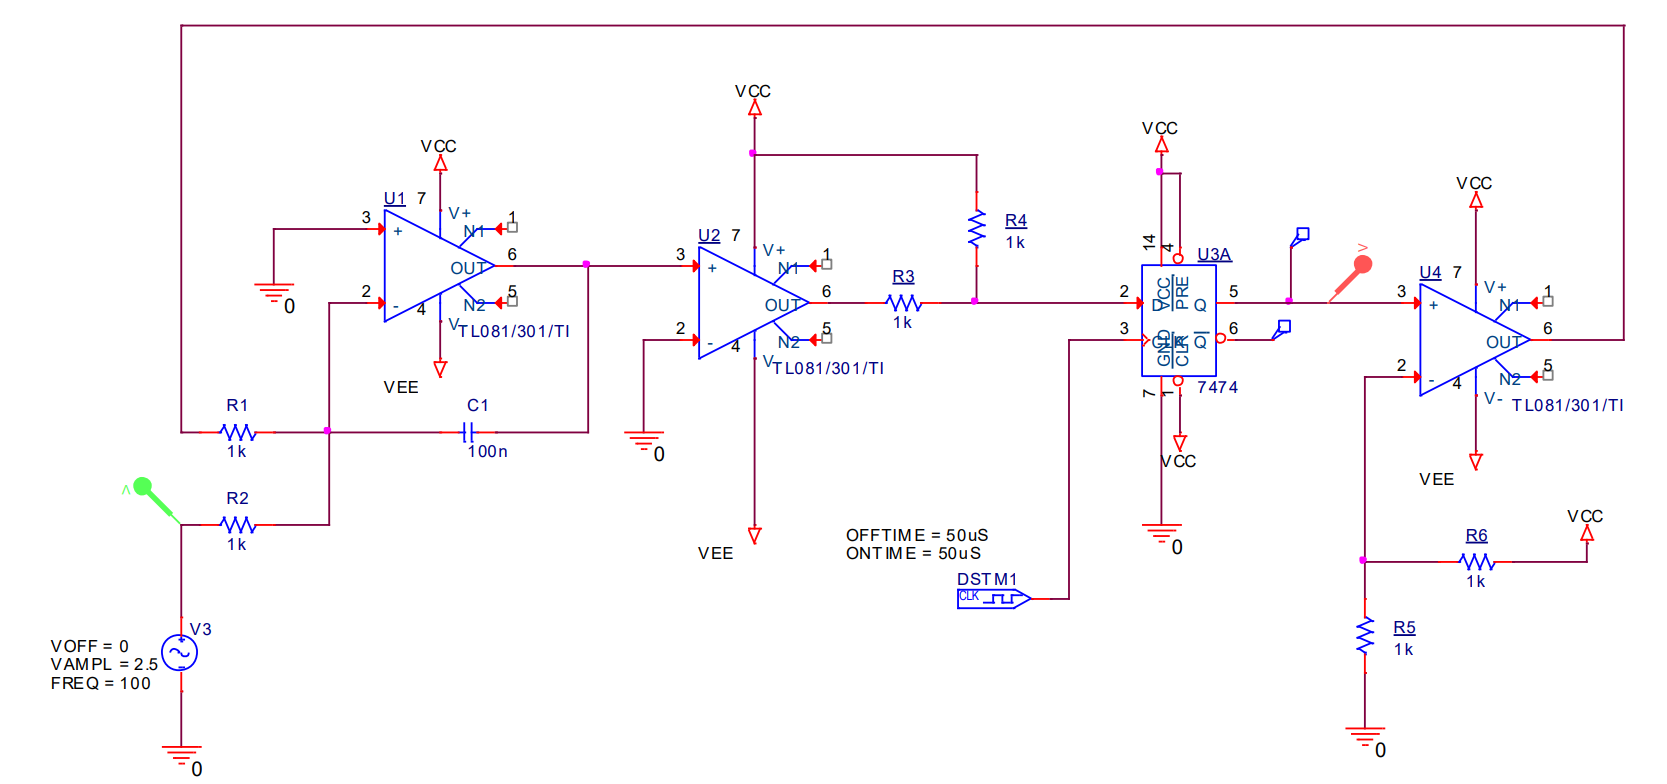
\includegraphics[width=\textwidth]{schem}
    \caption{Schema elettrico del circuito convertitore analogico digitale
    sigma-delta studiato \label{schm: ADC}}
\end{figure}
Con i canali 1 e 2 dell'oscilloscopio si osservano gli andamenti nel tempo del
segnale in ingresso e del segnale di uscita (OUT) dall'ultimo amplificatore
\verb+U4+, al contempo si registra il valore logico assunto dall'uscita $Q$
del Flip-Flop \verb+U3A+ con Logic (analyzer).

\subsection{Verifica del funzionamento}
Per verificare il corretto funzionamento del circuito si è inviata all'ingresso
analogico del circuito una sinusoide di bassa frequenza ($f = 10 \; \si{\Hz}
 \ll f\ped{clk}$) con ampiezza di $2.5 \; \si{\V}$ e media nulla.
Riportiamo l'acquisizione con l'oscilloscopio di qualche periodo dell'onda
sinusoidale su CH1 e dell'uscita di U4 su CH2 in \cref{fig: verif}.
\begin{figure}[htbp]
    \centering
	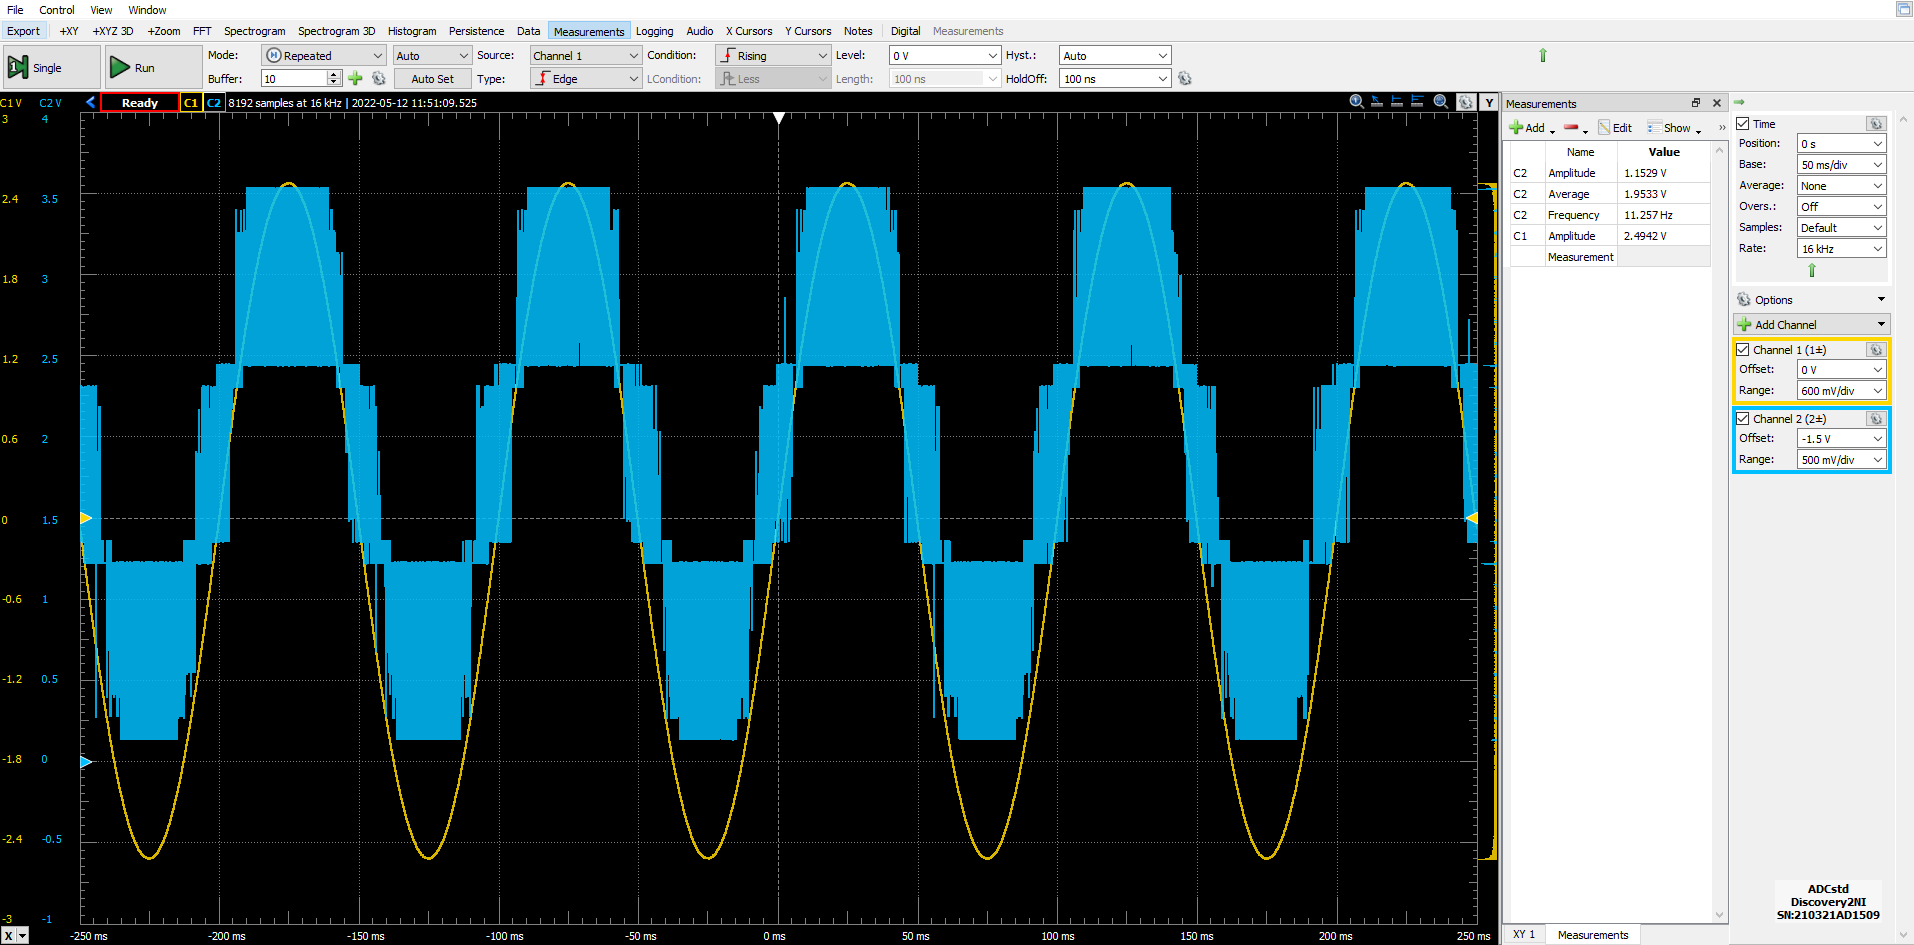
\includegraphics[width=\textwidth]{sin10hz2.5v}
    \caption{Acquisizione dell'andamento temporale del segnale in ingresso
    (CH1) e del segnale in uscita (CH2) dall'ADC
    \label{fig: verif}}
\end{figure}

\subsection{Analisi qualitativa del funzionamento del circuito}
Possiamo dividere il circuito in 3 sezioni principali: basandoci sullo schema mostrato in \cref{schm: ADC} individuiamo da sinistra verso destra un circuito sommatore e integratore invertente, un comparatore semplice e un flip flop che faranno da convertitore A->D a 1 bit, e infine un convertirore D->A anch'esso da 1 bit.
Il compito del sommatore e integratore è quello di fare la media nel tempo del segnale di feedback sommato a quello analogico in ingresso all'ADC, in modo che l'uscita dell'integratore sia >0 quando la media del segnale di feedback è inferiore a $V_{in}$ e viceversa.
L'uscita dell'integratore viene poi inviata all'ingresso di un comparatore la cui uscita sarà $V_{sat,+} \approx 3.5 V$ nel caso in cui l'uscita dell'integratore sia positiva, e $V_{sat,-} \approx -3.5 V$ nel caso opposto.
A questo punto si vuole modificare il segnale in modo che l'ingresso del flip flop possa interpretarlo correttamente come segnale digitale; per questo utilizzeremo un partitore di tensione tra l'uscita del comparatore e $V_{CC}$ in modo che H e L del segnale siano rispettivamente $4.25 V$ ( che risulta essere maggiore del valore nominale di $V_{IH}$) e $0.75 V$ (minore del valore nominale di $V_{IL}$).
L'uscita dal flip flop sarà quindi l'uscita digitale del nostro DAC.
Infine l'uscita digitale passerà attraverso un ultimo comparatore (che compara il segnale digitale con $2.5V$, e nel caso in cui sia maggiore, all'uscita avrò $V_{sat,+}$ e viceversa) che avrà la funzione di convertitore Digitale->Analogico ad un singolo bit, la cui uscita sarà inviata al circuito sommatore+integratore come segnale di feedback.
\begin{figure}[htbp]
    \centering
	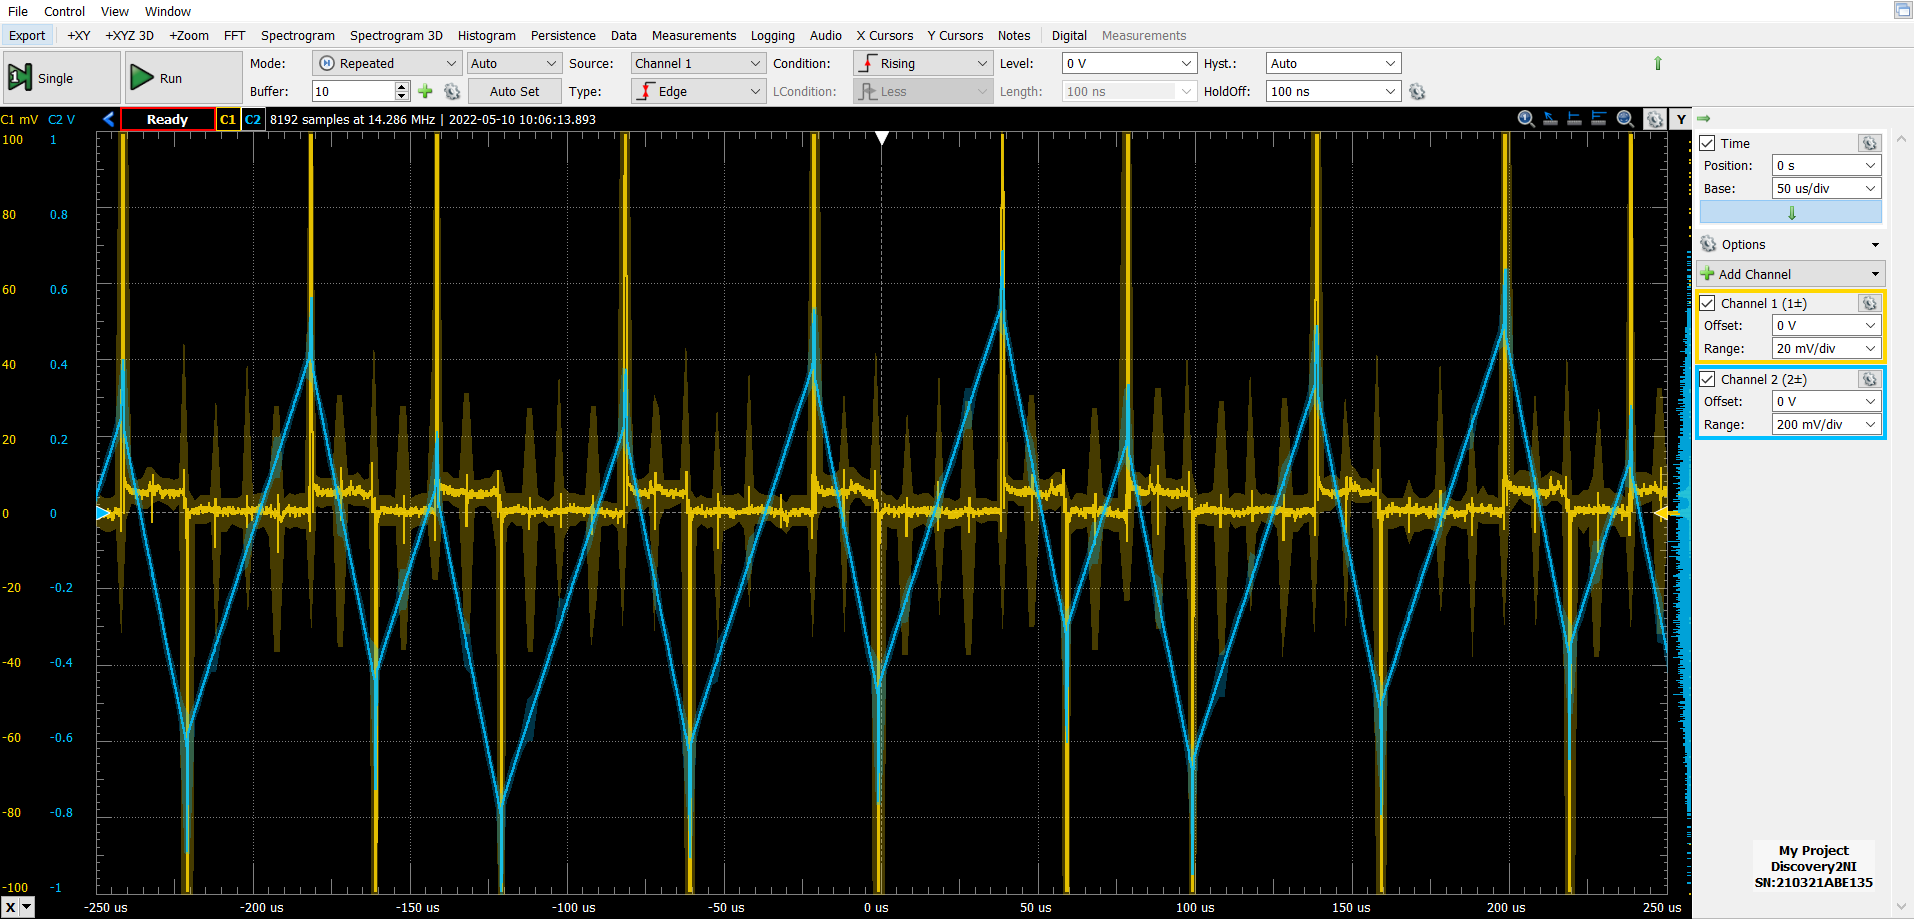
\includegraphics[width=\textwidth]{MIDDLE.U1.InputVSOutput}
    \caption{Acquisizione dei segnali all'ingresso invertente (CH1) e uscita (CH2)
    del circuito solo integratore \texttt{U1}}
\end{figure}

\begin{figure}[htbp]
    \centering
	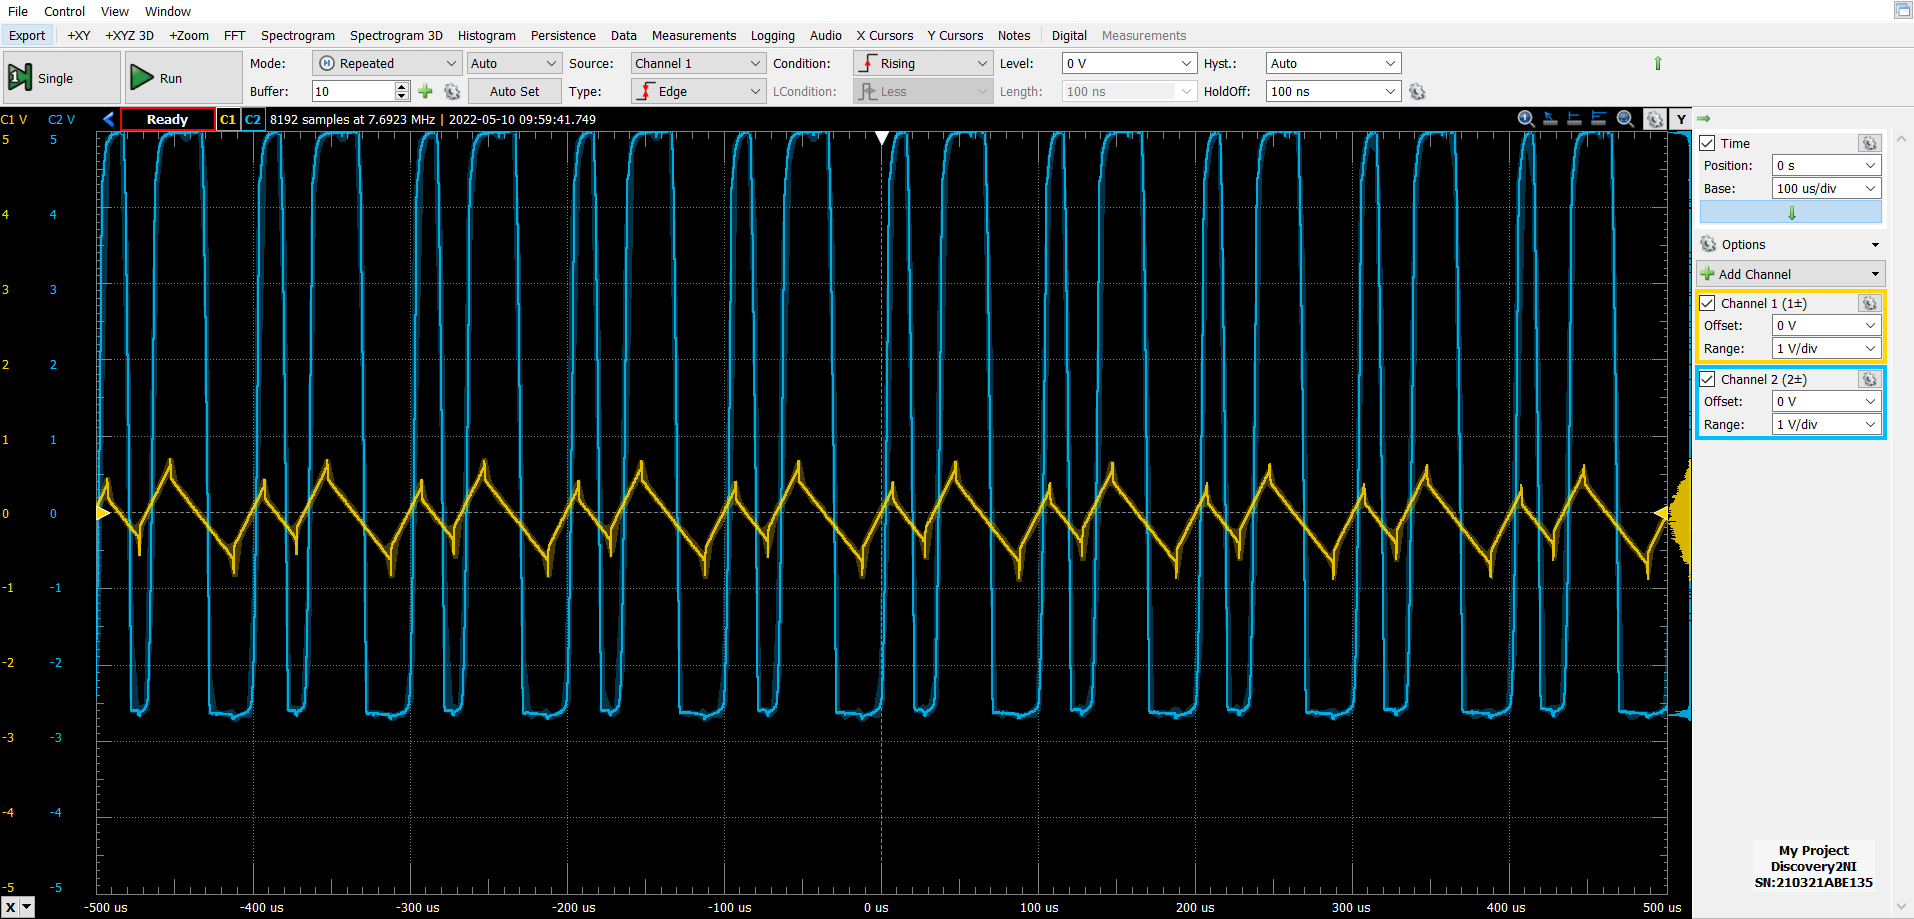
\includegraphics[width=\textwidth]{MIDDLE.U2.InputVSOutput}
    \caption{Acquisizione del segnale nell'ingresso non invertente (canale 1) e dell'uscita (canale 2) del circuito comparatore semplice}
\end{figure}
\begin{figure}[htbp]
    \centering
	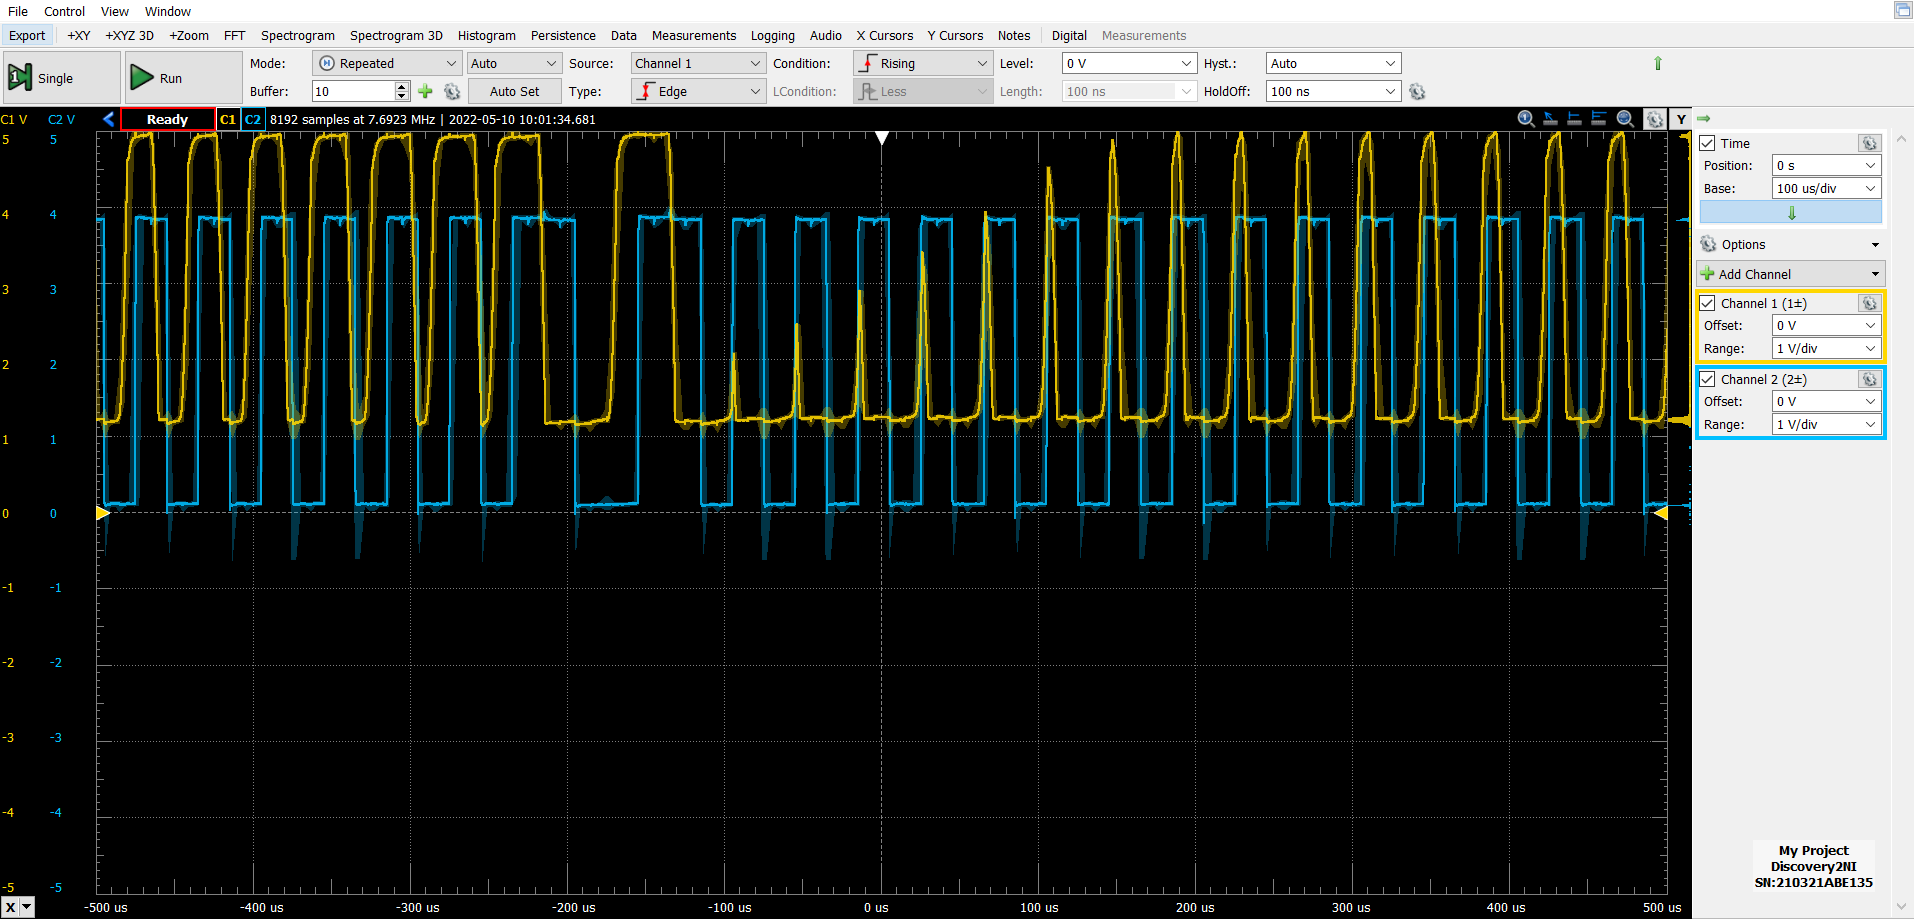
\includegraphics[width=\textwidth]{MIDDLE.U3.InputVSOutput}
    \caption{Acquisizione del segnale in ingresso(canale 1) e in uscita (canale 2) dal Flip Flop}
\end{figure}

\begin{figure}[htbp]
    \centering
	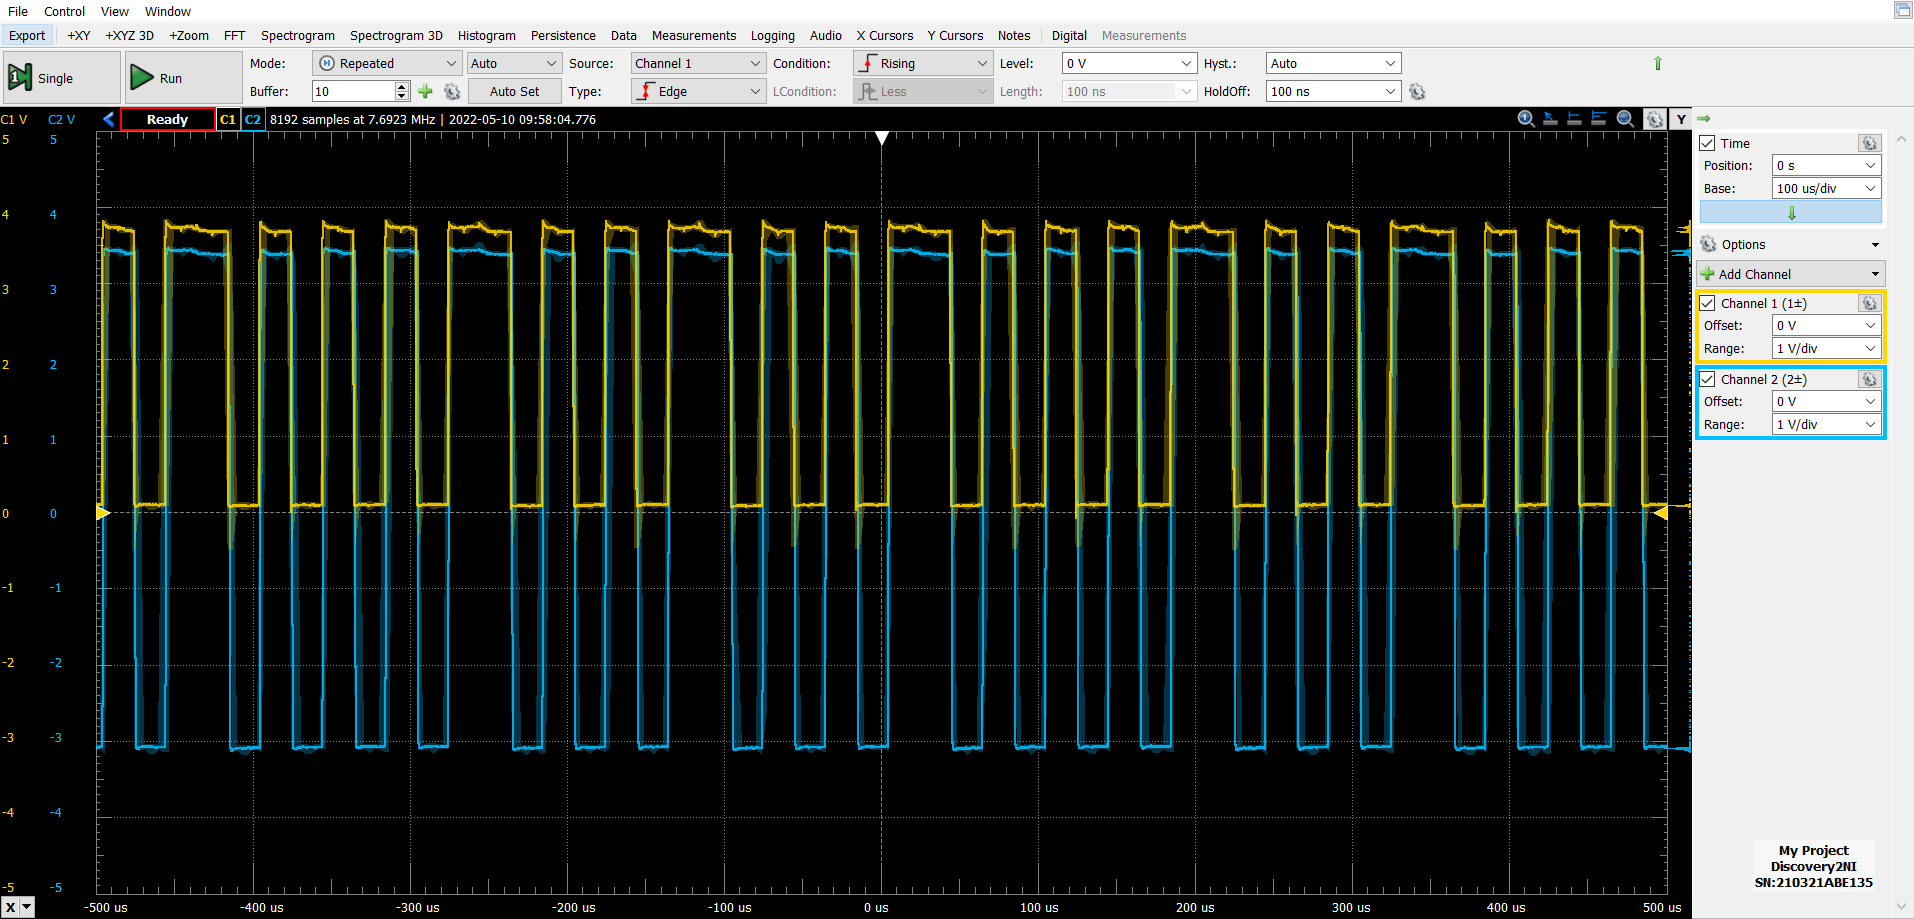
\includegraphics[width=\textwidth]{MIDDLE.U3vU4}
    \caption{Acquisizione del segnale in uscita dal pin Q del Flip Flop(canale 1) e in uscita dal DAC (canale 2)}
\end{figure}
Dalle acquisizioni fatte con l'oscilloscopio di Waveform, ci accorgiamo che ogni componente del circuito si comporta come atteso.
Si procede quindi alla verifica del funzionamento del convertitore A->D: per farlo, dopo aver alimentato ogni componente del circuito, inviamo un segnale di clock al flip flop di frequenza pari a 50 kHz, e un'onda sinusoidale di ampiezza $2.5 V$ e frequenza $10 Hz$ all'entrata analogica; ci concentriamo quindi sui segnali in uscita dal Flip Flop.
Dopo ciò che si è detto prima, ci aspettiamo in uscita dal flip flop un segnale simile ad un'onda quadra con duty cycle medio $\approx 50 \percent$ quando l'onda vale circa 0 V, e che il Duty Cycle aumenti quando l'onda raggiunge il minimo e viceversa.
\begin{figure}[htbp]
    \centering
	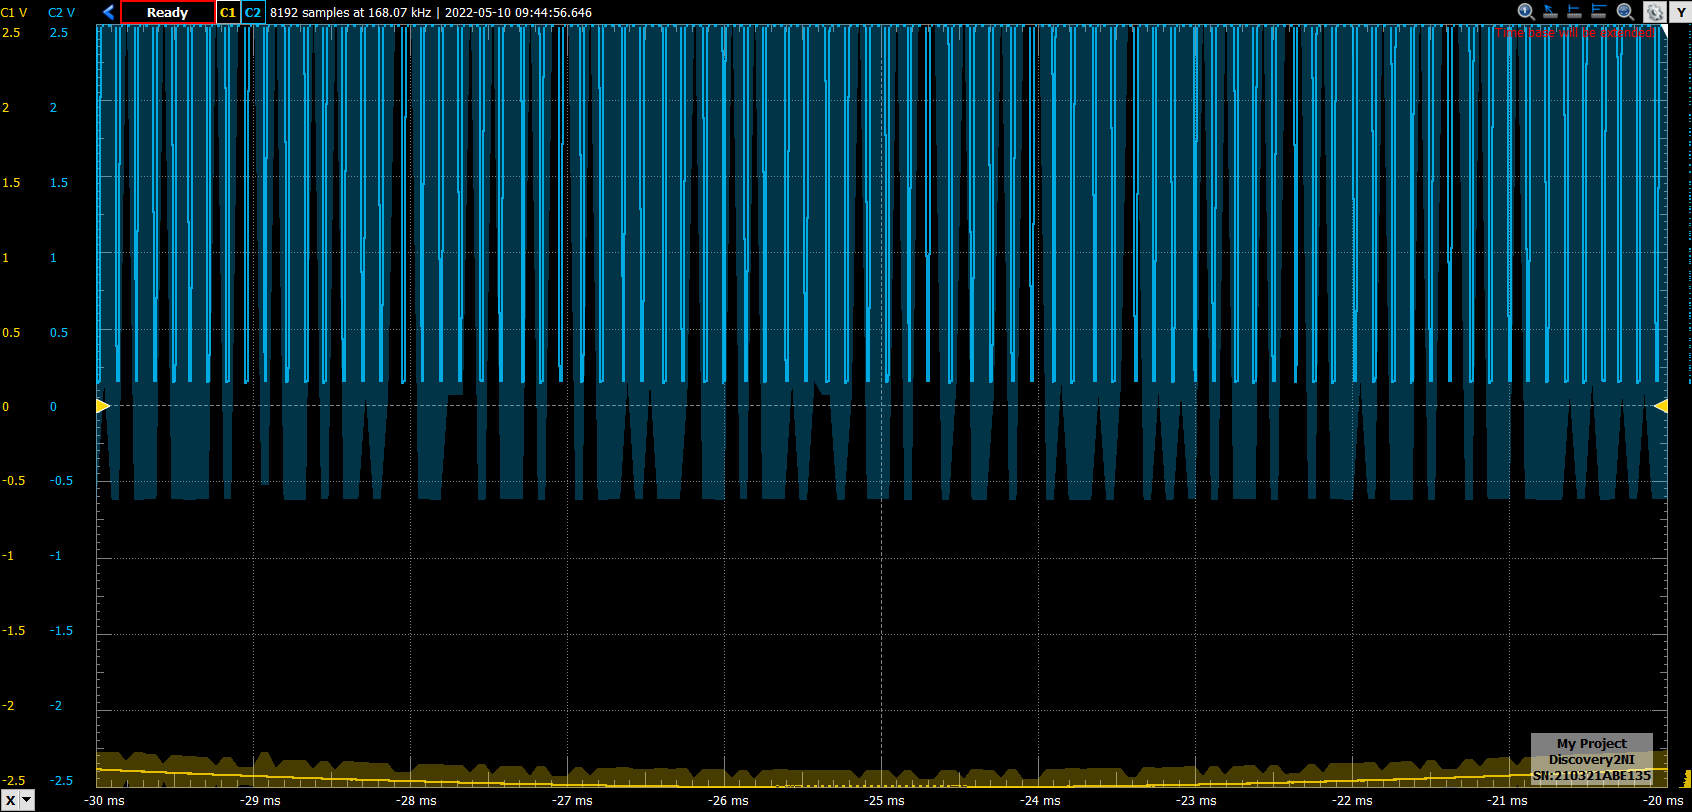
\includegraphics[width=\textwidth]{BOTTOM}
    \caption{Acquisizione del segnale analogico in ingresso (un'onda sinusoidale di frequenza pari a 10 Hz e ampiezza pari a $2.5 V$) e del segnale logico in uscita dal pin Q del Flip-Flop durante il minimo del segnale}
\end{figure}
\begin{figure}[htbp]
    \centering
	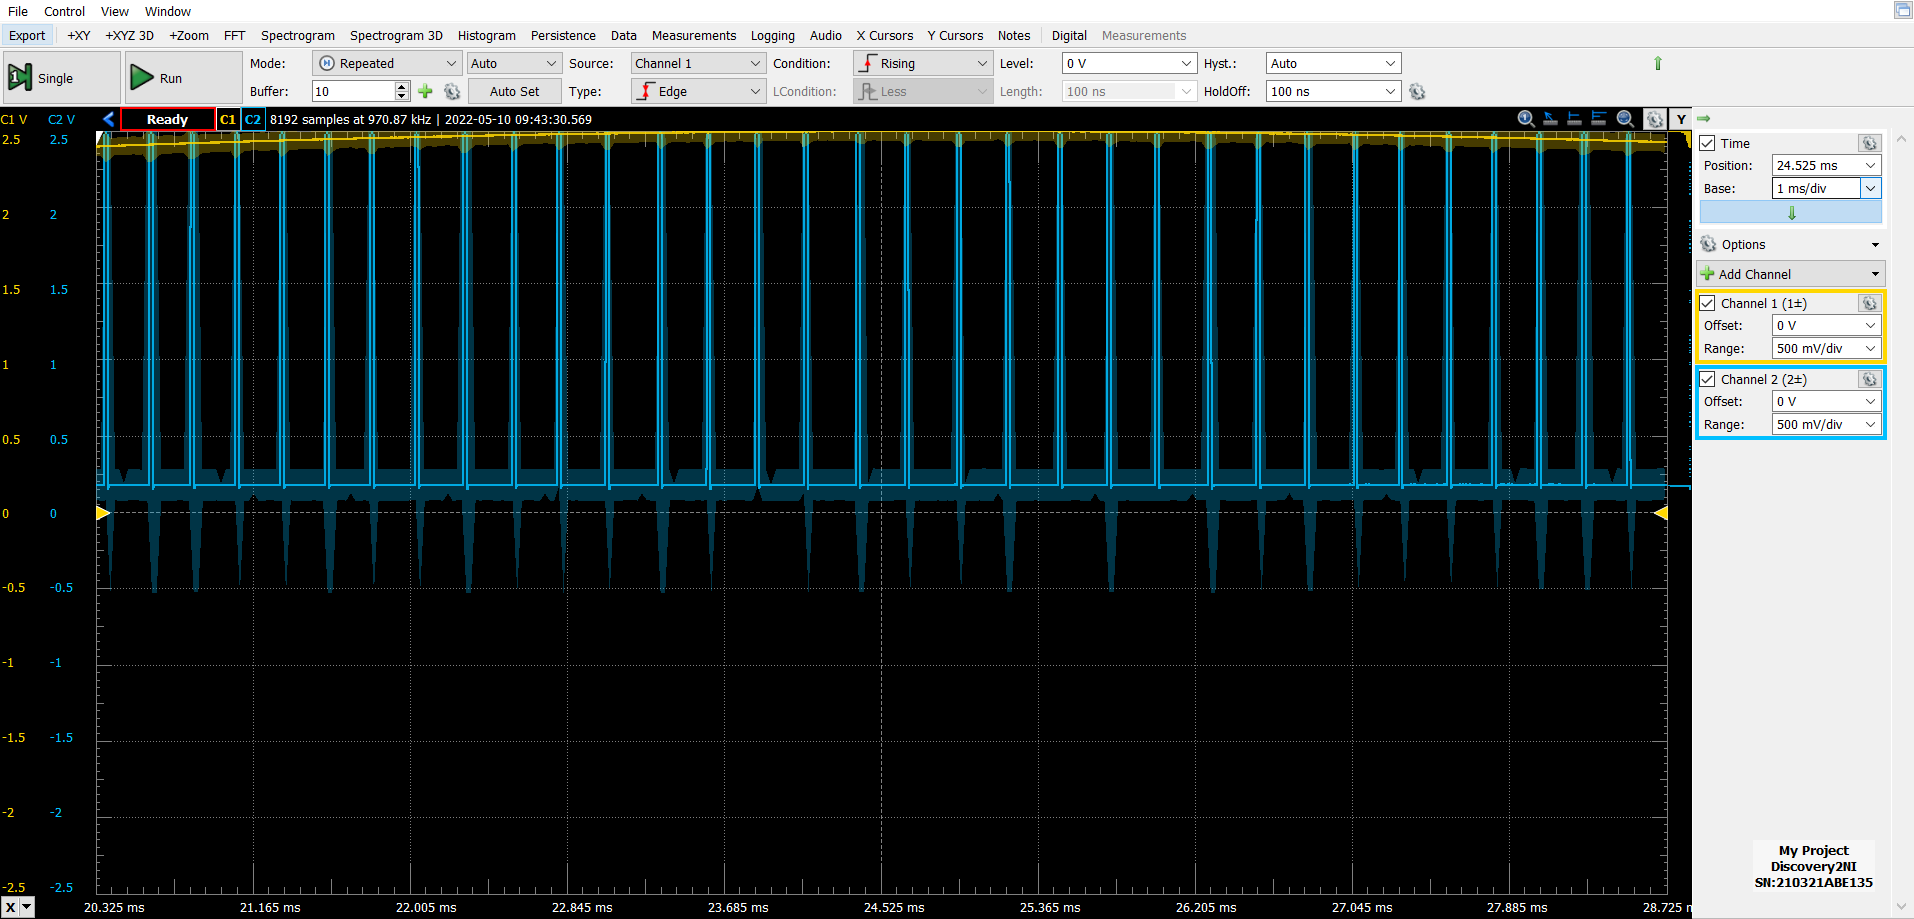
\includegraphics[width=\textwidth]{TOP}
    \caption{Acquisizione del segnale analogico in ingresso (un'onda sinusoidale di frequenza pari a 10 Hz e ampiezza pari a $2.5 V$) e del segnale logico in uscita dal pin Q del Flip-Flop durante il massimo del segnale}
\end{figure}
\begin{figure}[htbp]
    \centering
	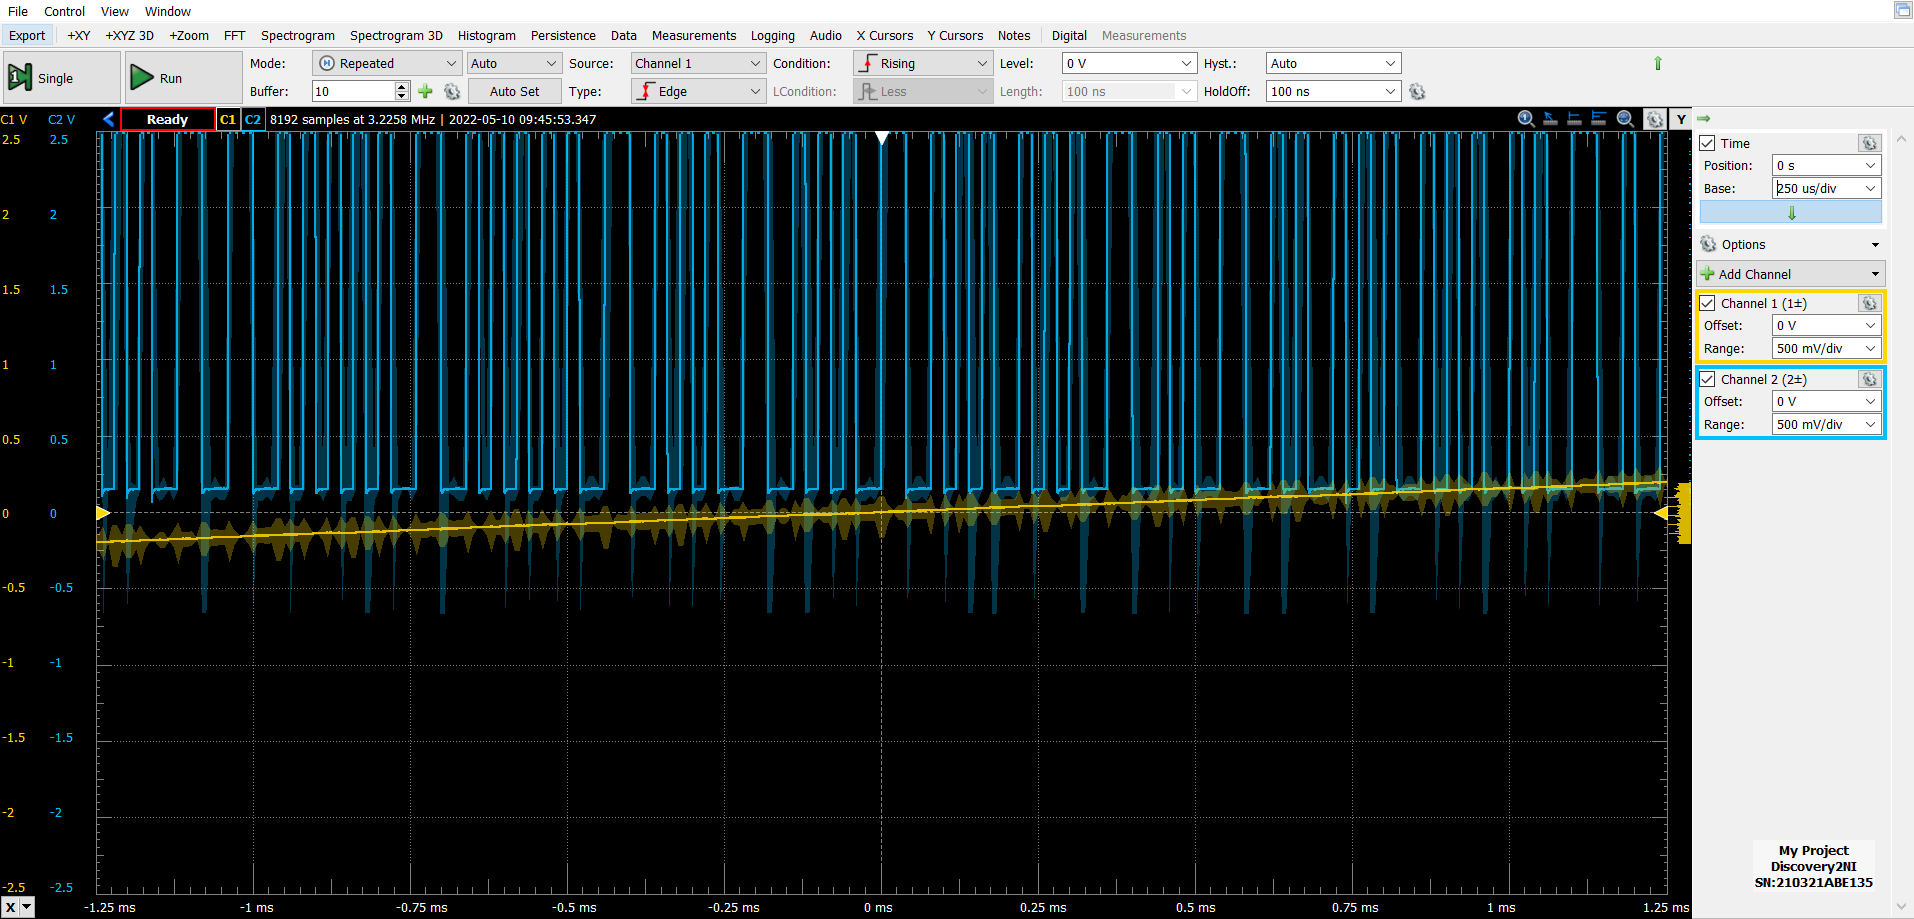
\includegraphics[width=\textwidth]{MIDDLE}
    \caption{Acquisizione del segnale analogico in ingresso (un'onda sinusoidale di frequenza pari a 10 Hz e ampiezza pari a $2.5 V$) e del segnale logico in uscita dal pin Q del Flip-Flop durante il punto medio dell'onda}
\end{figure}
Dalle acquisizioni possiamo concludere che il circuito ha il comportamento atteso
\subsection{Risposta del convertitore al variare dei parametri del seno}
\label{sbs: adcresp}
Modificando i valori di offset e ampiezza dell'onda in ingresso si nota
immediatamente come il segnale in uscita venga tosato ai livelli di
saturazione basso $V_{OL} = 138 \pm 2 \; \si{m\V}$ e alto
$V_{OH} = 3.52 \pm 0.02 \; \si{\V}$ quando il segnale in ingresso raggiunge
valori di tensione pari a circa $V_s \approx \pm 3 \; \si{\V}$ per via della
portata limitata del nostro convertitore.

Si riporta la risposta del circuito per un'onda della stessa ampiezza (2.5 V)
e offset = 2 V in \cref{fig: sinofs}
\begin{figure}[htbp]
    \centering
	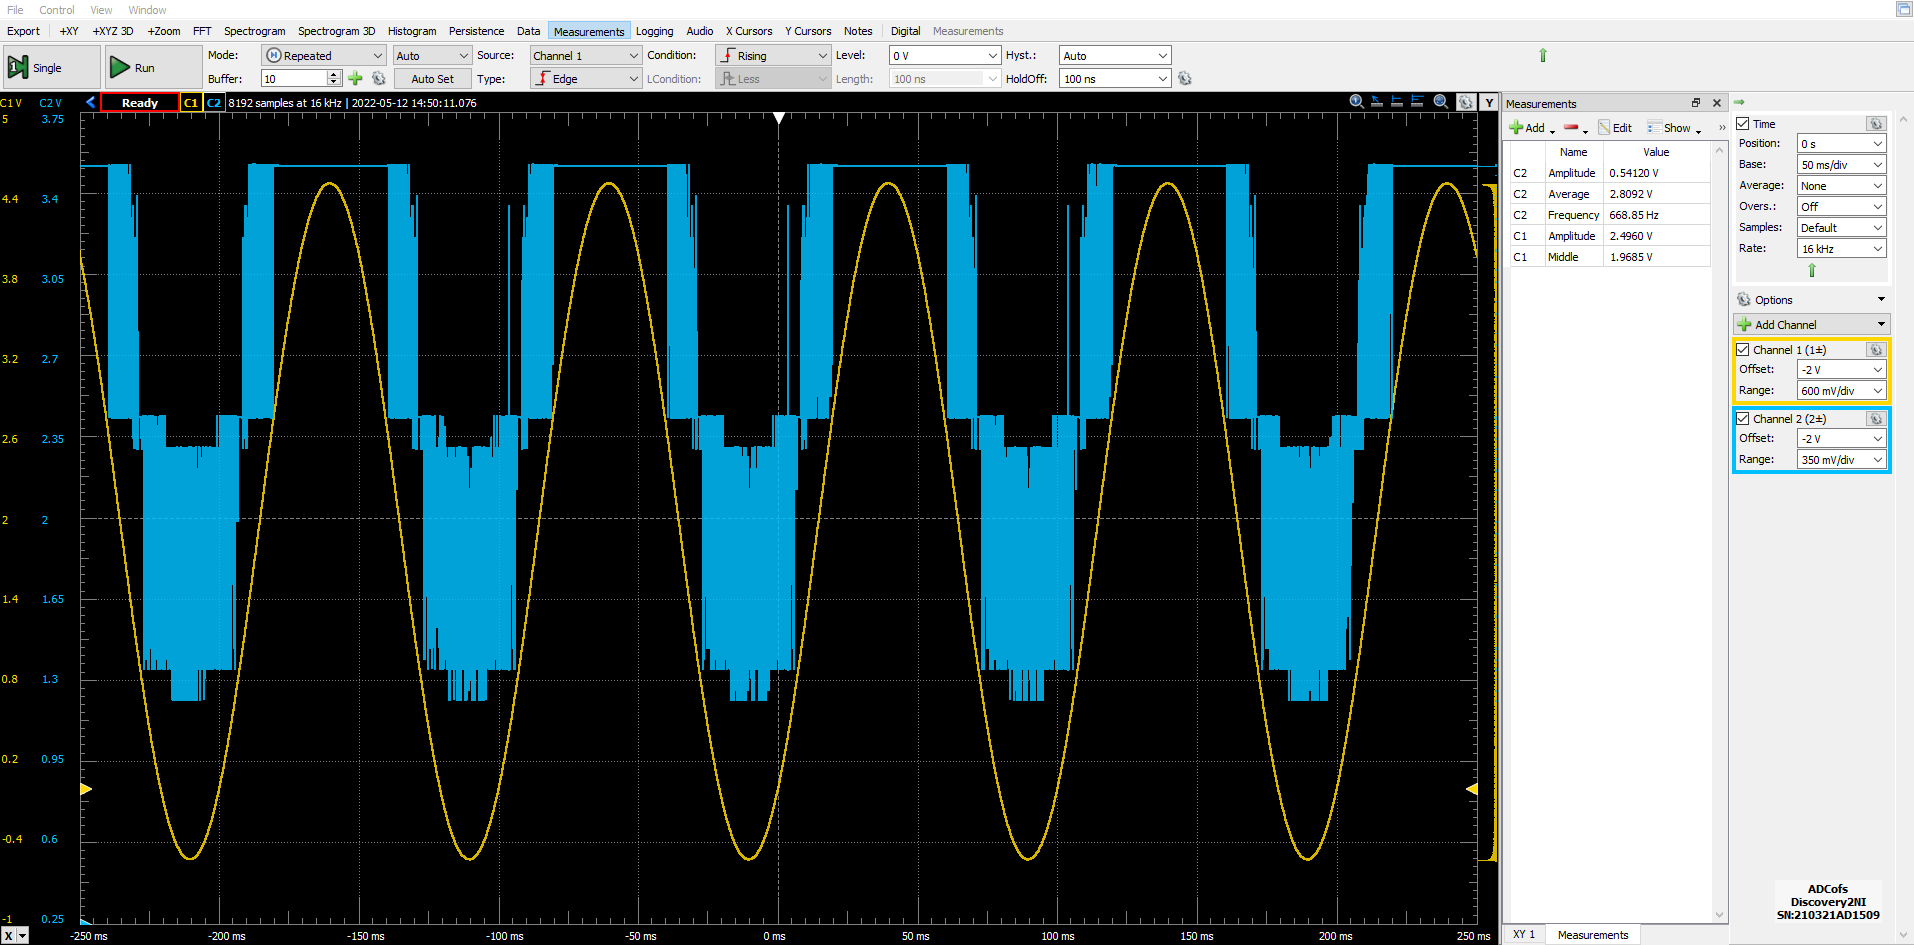
\includegraphics[width=\textwidth]{sin10hz2.5vofs2v}
    \caption{Acquisizione dell'andamento temporale del segnale in ingresso
    (CH1) e del segnale in uscita (CH2) dall'ADC
    \label{fig: sinofs}}
\end{figure}
e per un'onda di ampiezza maggiore (5 V) e offset = 0 V in \cref{fig: sinsat}.
\begin{figure}[htbp]
    \centering
	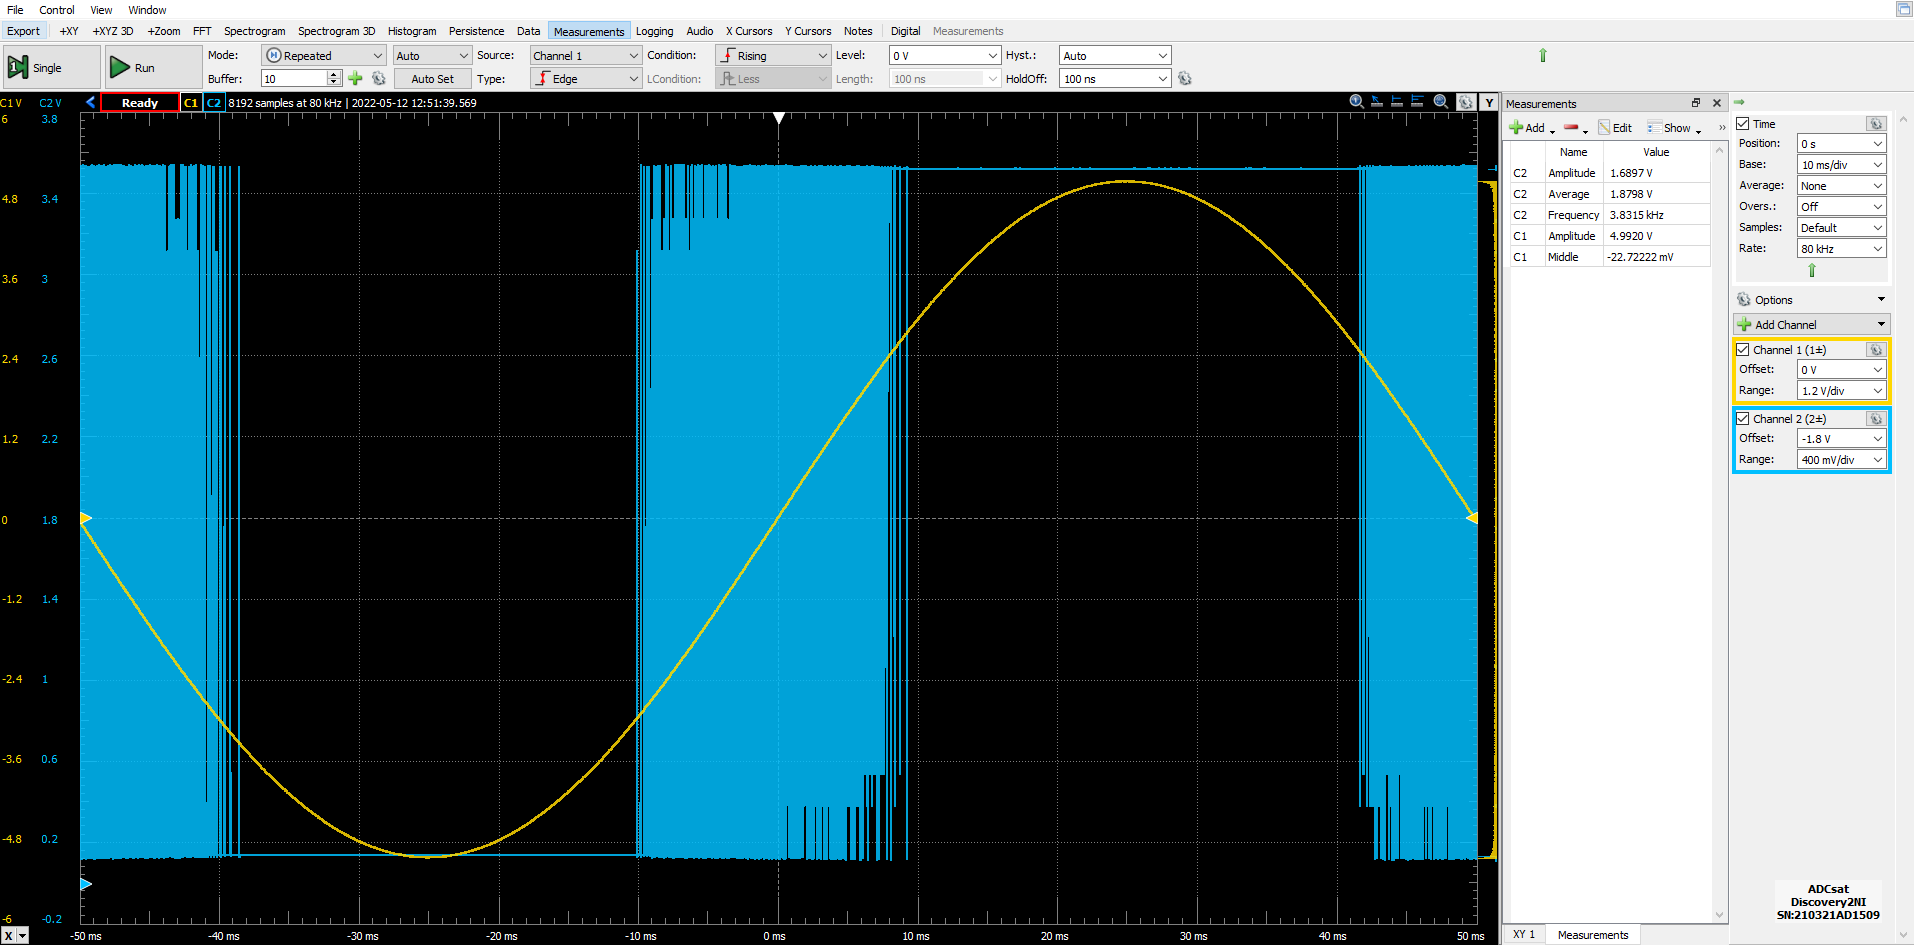
\includegraphics[width=\textwidth]{sin10hz5v}
    \caption{Acquisizione dell'andamento temporale del segnale in ingresso
    (CH1) e del segnale in uscita (CH2) dall'ADC
    \label{fig: sinsat}}
\end{figure}

Quanto trovato risulta compatibile con il massimo intervallo di tensioni che
il segnale analogico di ingresso può assumere senza rischiare saturazioni nel
nostro circuito $\approx 7$ V, assumendo che il valore di uscita del nostro
DAC risulti essere $-V\ped{sat}$ in corrispondenza di uno 0 logico e
$V\ped{sat} \approx 3.5$ V in corrispondenza di un 1.

Aumentando la frequenza $f$ del segnale in ingresso al circuito si nota come
l'informazione in uscita sull'onda da ricostruire (proporzionale al numero di
punti campionati/alla densità di fronti d'onda) diminuisce man mano che $f$ si
avvicina alla frequenza massima di campionamento $f\ped{clk}$, come si mostra
in \cref{fig: sin100hz} per $f = 100 \; \si{\Hz}$.
\begin{figure}[htbp]
    \centering
	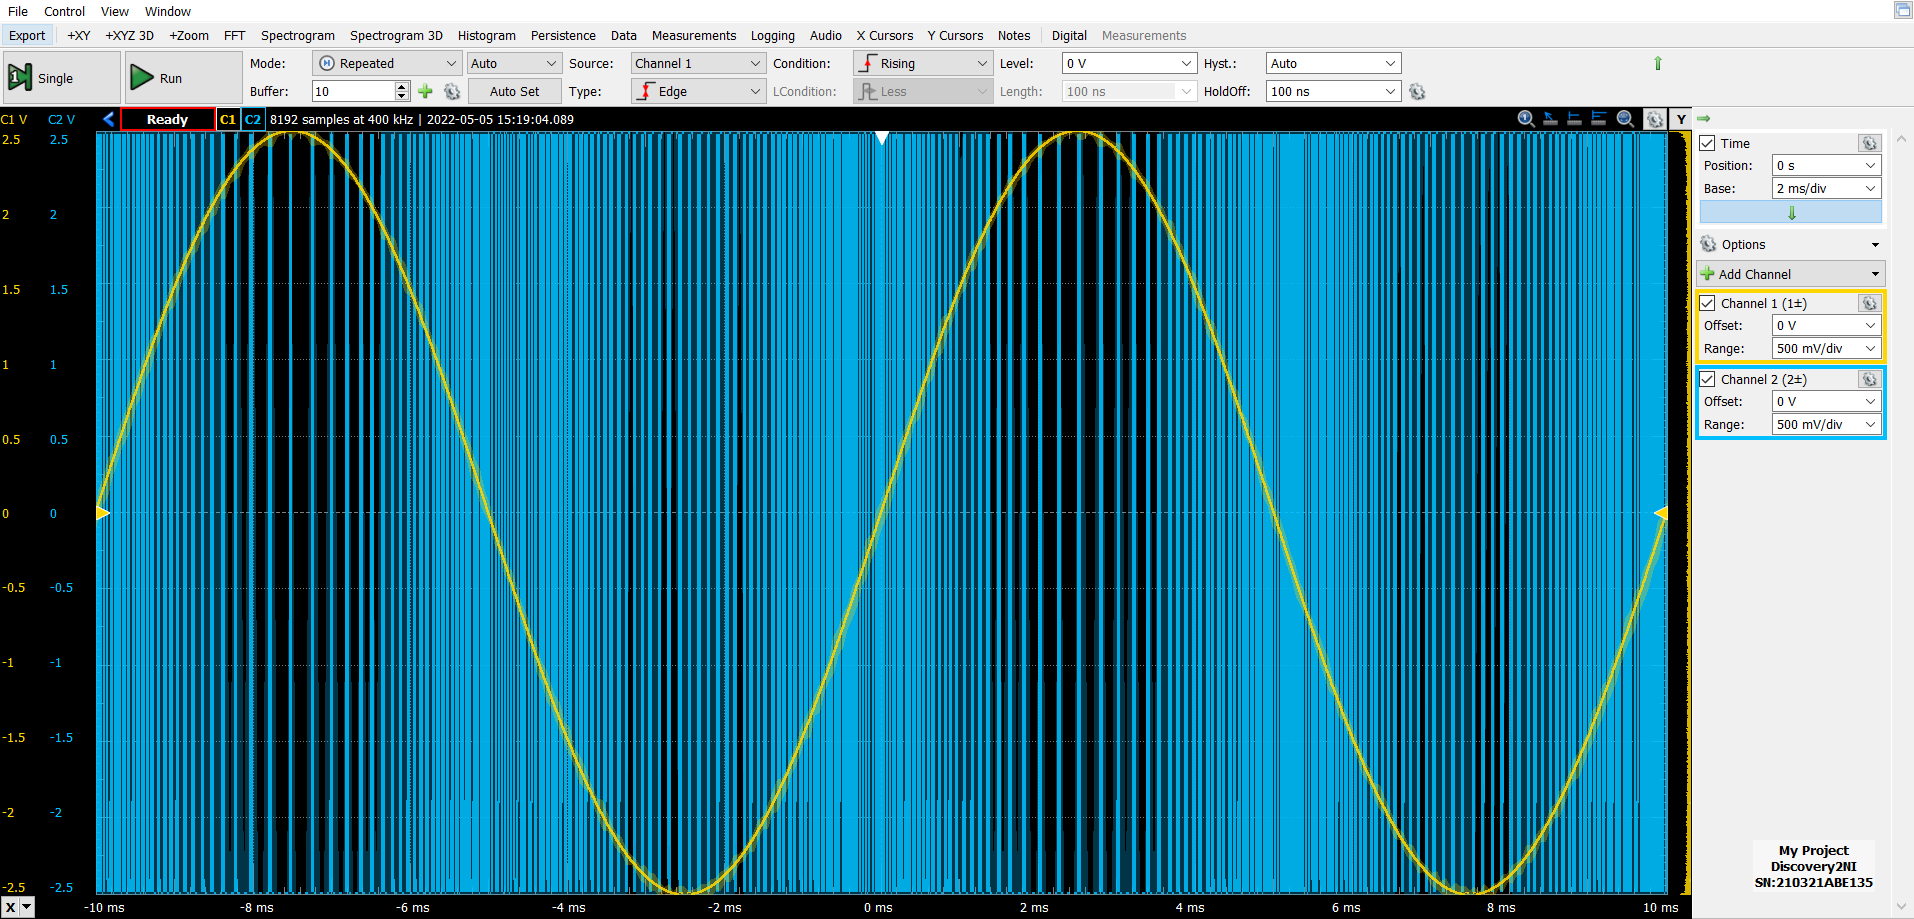
\includegraphics[width=\textwidth]{Conv.Sinusoide.100Hz.2}
    \caption{Acquisizione del segnale sinusoidale in ingresso (CH1)
    $f = 100$ Hz e ampiezza $2.5$ V e del segnale in uscita dal DAC (CH2)
    \label{fig: sin100hz}}
\end{figure}
e in \cref{fig: sin2khz} per $f = \SI{2}{k\Hz}$.
\begin{figure}[htbp]
    \centering
	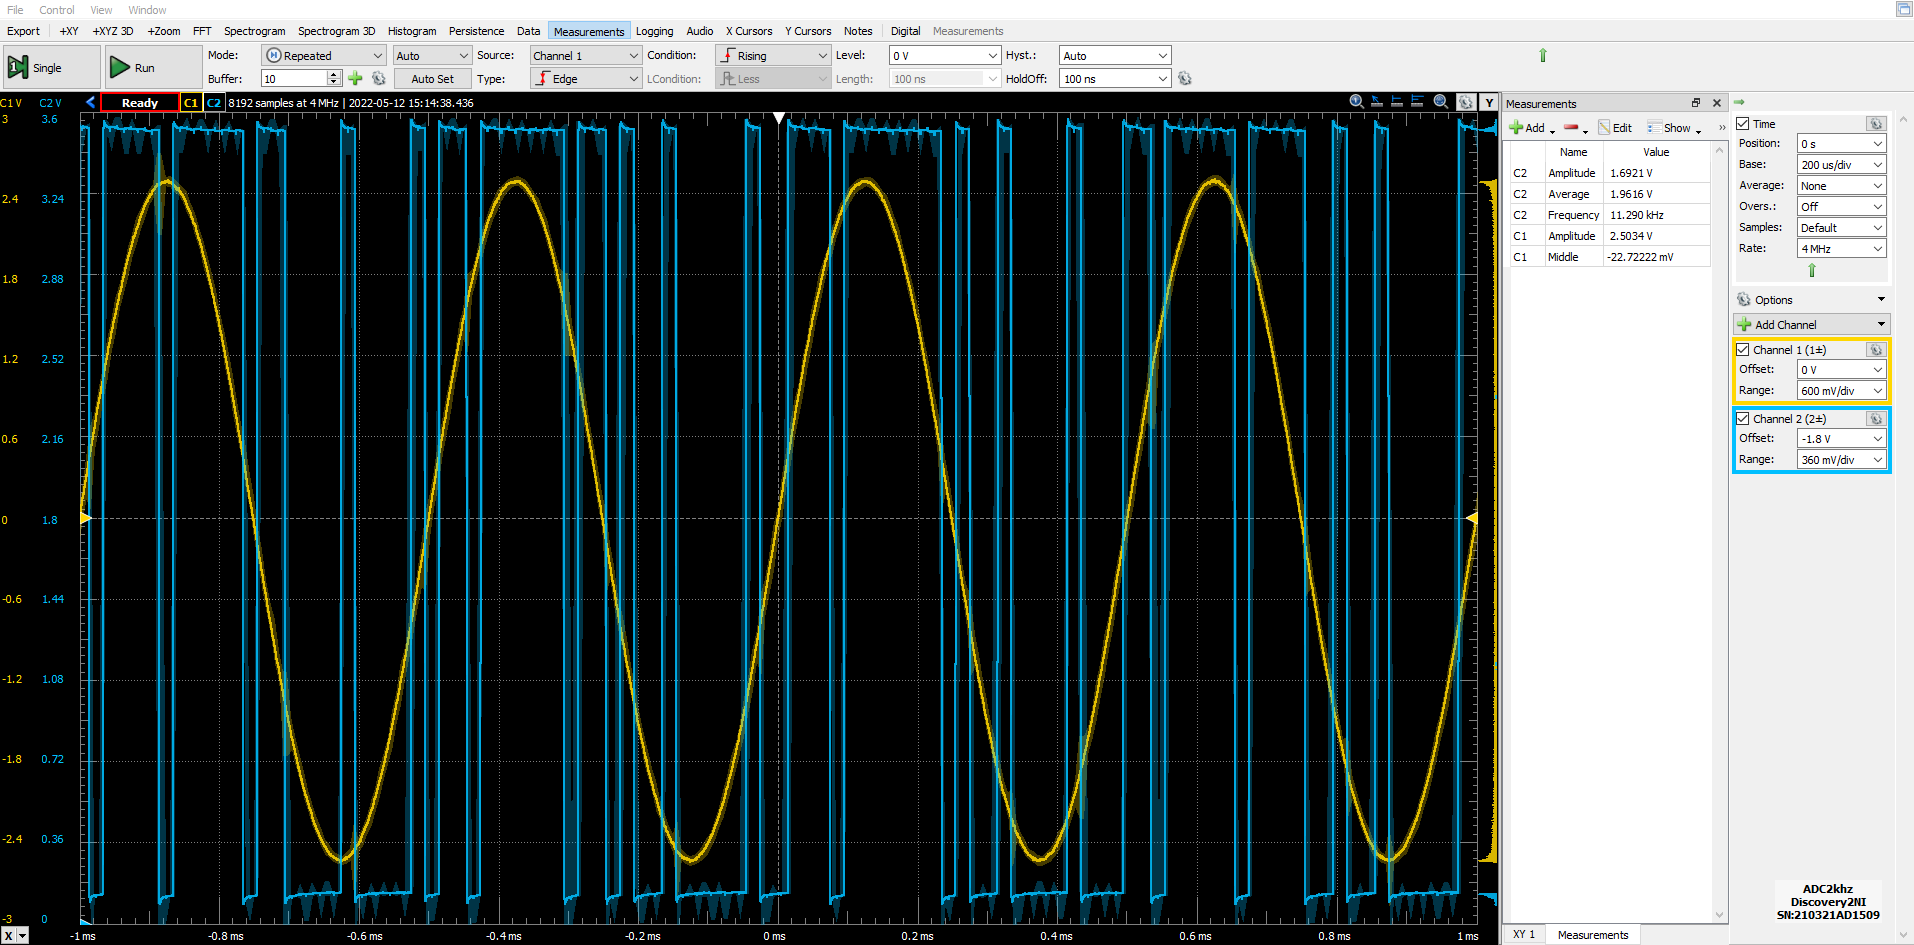
\includegraphics[width=\textwidth]{sin2khz2.5v}
    \caption{Acquisizione del segnale sinusoidale in ingresso (CH1)
    $f = 2$ kHz e ampiezza $2.5$ V e del segnale in uscita dal DAC (CH2)
    \label{fig: sin2khz}}
\end{figure}

Questo risulta compatibile con quanto ci aspettiamo per via della risoluzione
temporale limitata (proprio dalla frequenza di clock) del nostro modulatore
delta. Infatti, per ripristinare la densità di informazione che avevamo su
segnali più lenti, è sufficiente aumentare proporzionalmente la frequenza
di clock/campionamento inviata con DIO 0 al FF.

%=======================
\section{Descrizione delle misure e acquisizione dati}
\subsection{Campionamento e acquisizione del segnale}
Per acquisire il segnale in uscita dal Flip-Flop con l'AD2 si sono reimpostate
la frequenza della sinusoide in ingresso a $f = 100 \; \si{\Hz}$ e la
frequenza del clock come prima a $f\ped{clk} = 50 \; \si{k\Hz}$, dunque
leggiamo in modalità Spy un bus SPI creato con lo strumento Protocol di
Waveforms, impostando i parametri come segue:
\begin{description}
\item[Select:] None
\item[Frequency:] 50 kHz (come il clock in DIO 0)
\item[Clock:] DIO 0
\item[Data:] DIO 1
\item[Mode:] Three-wire
\item[Data bits:] 8
\item[Format:] Decimal
\end{description}

Si registrano una decina di periodi della sinusoide lasciando lo strumento in
modalità Receive per qualche frazione di secondo, quindi salviamo la serie
di valori campionati su file di testo per analizzarli e ricostruire il segnale
in ingresso.

%=======================
\section{Analisi dei dati}
\subsection{Ricostruzione dei segnali in ingresso}
Come abbiamo visto, il segnale in uscita dal Flip-Flop $Q$ commuta in
corrispondenza dei fronti di salita del clock l'ampiezza del segnale in
ingresso è proporzionale alla densità relativa di bit a livello logico alto
nella sequenza in OUT. Quindi per ricostruire l'ampiezza del segnale possiamo
effettuare un conteggio di quanti bit sono in stato $1$ nella sequenza in
uscita da Protocol in un intervallo di tempo con una media mobile su $8$ bit.

Riportiamo in \cref{fig: sin100hzpy} la forma d'onda ottenuta su un grafico
con Python, in cui i punti blu rappresentano i valori digitali in uscita dal
DAC, i punti in giallo sono il risultato della prima operazione di media
mobile a 8 bit e i punti in verde il risultato dopo una seconda operazione di
media mobile sempre a 8 bit e decimati di un fattore pari a 8.
\begin{figure}[htbp]
    \centering
	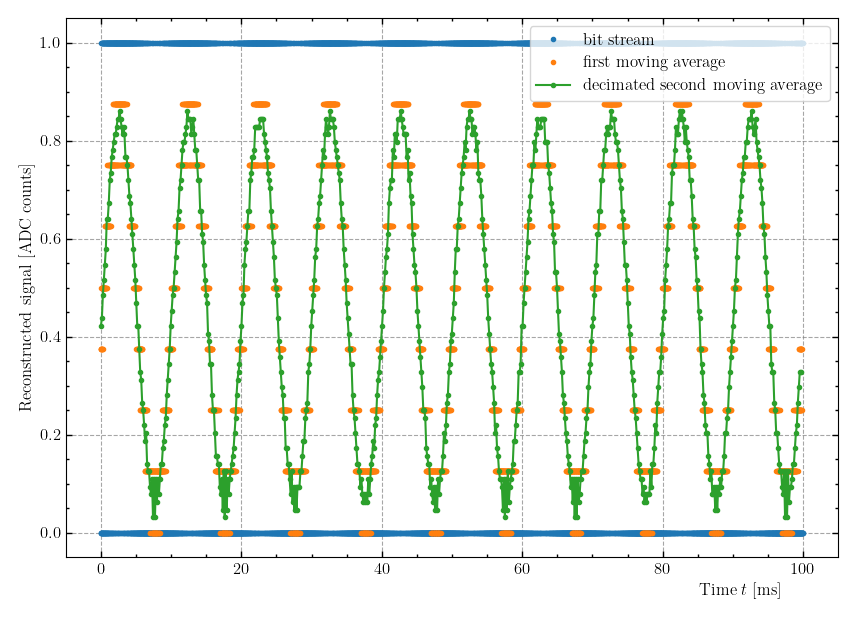
\includegraphics[width=\textwidth]{recsin}
    \caption{Ricostruzione del segnale sinusoidale in ingresso di $f = 100$
    Hz e ampiezza $2.5$ V a partire dall'acquisizione del segnale in uscita
    dall'ADC con Protocol.
    \label{fig: sin100hzpy}}
\end{figure}

\subsection{Fit sinusoidale}\label{sbs: sinfit}
Si è effettuato un fit con un legge della forma $A\sin(2\pi f t + \phi) + B$
\begin{lstlisting}[language=Python]
def sin(t, A, f, phi, B):
    return A*np.sin(2*np.pi*f*t + phi) + B
\end{lstlisting}

lasciando liberi tutti i parametri, da cui si ottengono il grafico riportato 
in \cref{fig: sinfit}
\begin{figure}[htbp]
    \centering
	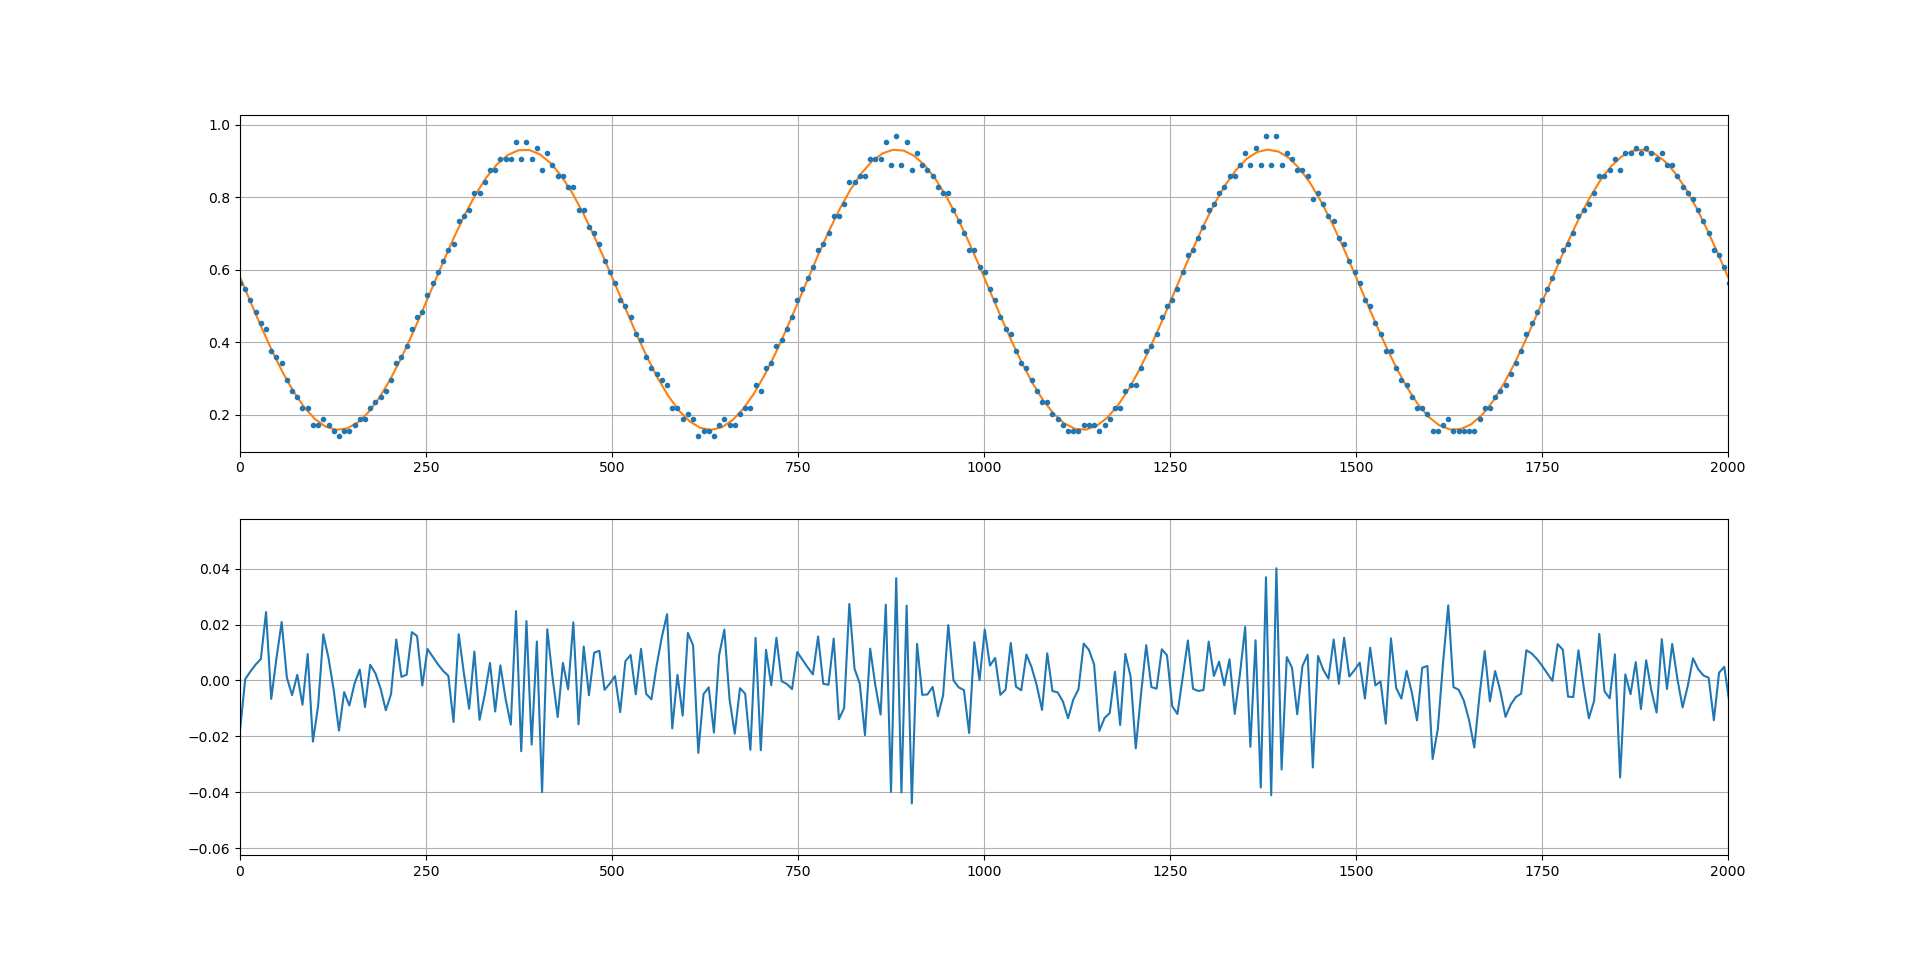
\includegraphics[width=\textwidth]{sinfit}
    \caption{Grafico del fit con una forma d'onda sinusoidale e dei residui
    per l'andamento nel tempo dei punti campionati e ricostruiti dal secondo ADC.
    \label{fig: sinfit}}
\end{figure}
e come stime dei valori ottimali:
\begin{align*}
A &= 404 \times 10^{-3} \pm 2 \times 10^{-4} \quad f = 99.9\pm 7 \times 10^{-5}\; \si{Hz} \\
B &= 545 \times 10^{-3} \pm 1 \times 10^{-4} \quad \phi = -0.09 \pm \; 7 \times 10^{-4}\si{rad} \\
\chi^2/\text{d.o.f} &=  4 / 20554
\end{align*}

\subsection{Risposta in frequenza dell'ADC}
\label{sbs: freq}
Come visto in \cref{sbs: adcresp} il convertitore studiato riesce a funzionare
correttamente per segnali in ingresso fino a frequenze dell'ordine di qualche
kHz; oltre cui la forma d'onda ricostruita in uscita risulta affetta da
aliasing per via del basso numero di punti campionati lungo un periodo del
segnale in ingresso.

Riportiamo quindi in \cref{fig: sin2khzpy} la ricostruzione ottenuta per lo
stesso segnale sinusoidale di frequenza $f = \SI{2}{k\Hz}$ (visualizzato
all'oscilloscopio prima in \cref{fig: sin2khz}) e in \cref{fig: net}
la risposta in frequenza all'uscita U4 del circuito ottenuta da uno scan con
Network Analyzer inviando una sinusoide di ampiezza fissata a $2.5 \; \si{\V}$
e frequenza tra $100$ e $\SI{10}{k\Hz}$ all'ingresso analogico dello stesso.
\begin{figure}[htbp]
    \centering
	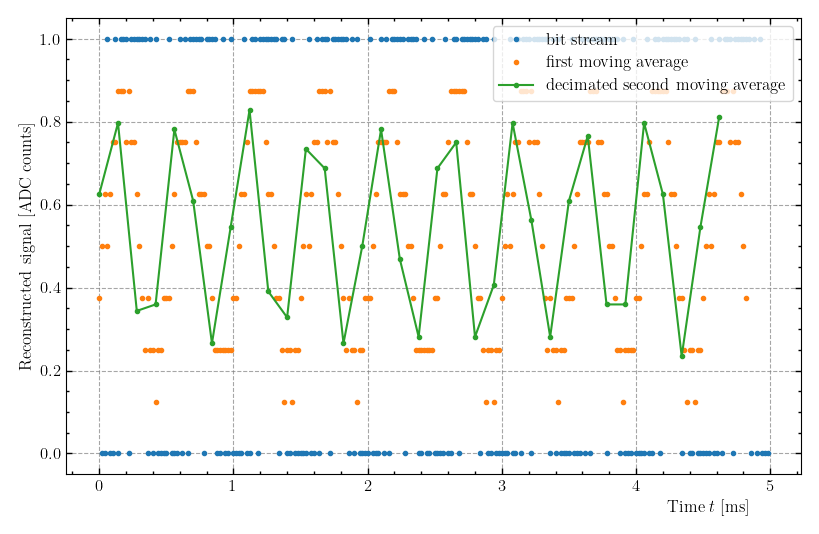
\includegraphics[width=\textwidth]{sin2khzpy}
    \caption{Ricostruzione del segnale sinusoidale in ingresso di $f = 2$
    kHz e ampiezza $2.5$ V a partire dall'acquisizione del segnale in uscita
    dall'ADC con Protocol.
    \label{fig: sin2khzpy}}
\end{figure}
\begin{figure}[htbp]
	\centering
	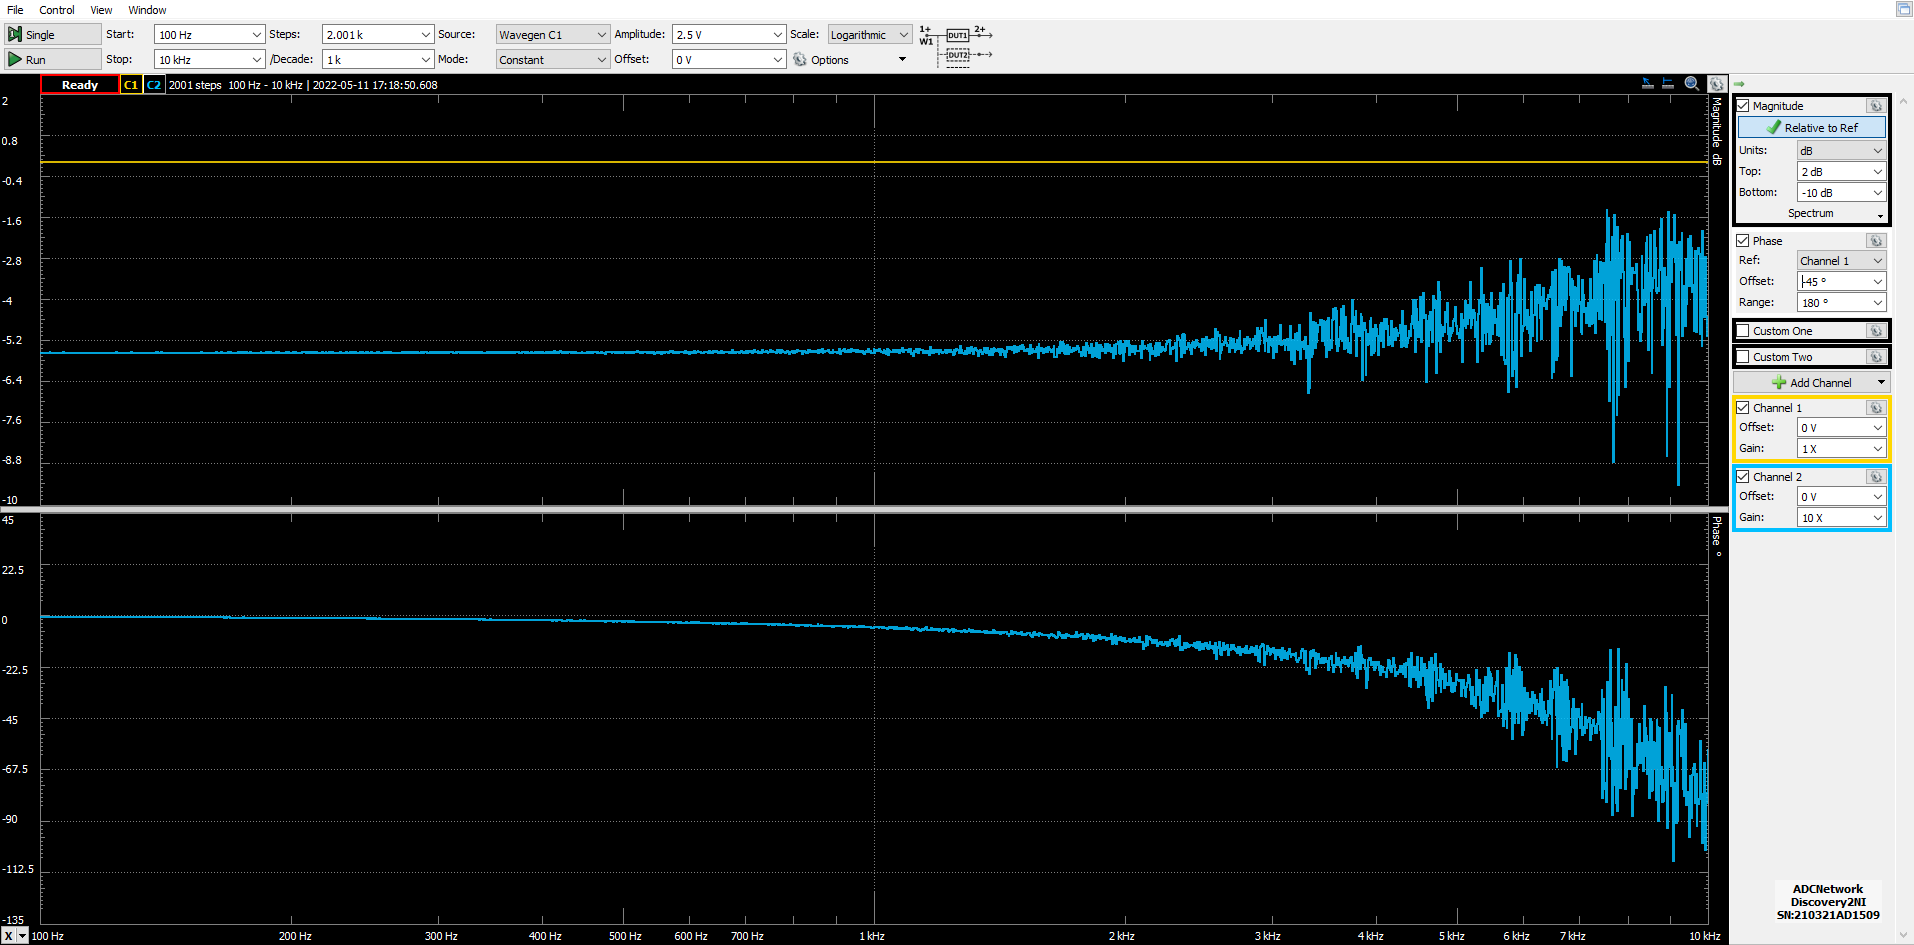
\includegraphics[width=\textwidth]{Net100-10k}
	\caption{Analisi in frequenza dell'ADC ottenuta dallo scan con Network
	tra $\SI{100}{\Hz}$ e $\SI{10}{k\Hz}$ con segnale sinusoidale in ingresso
	di ampiezza fissata a $v\ped{in} = 2.5 \; \si{\V}$. L'unico punto di
	interesse si trova a circa $\SI{2}{k\Hz}$, frequenza oltre alla quale il
	circuito assume un comportamento irregolare. L'andamento della fase risulta
	qualitativamente simile a quello atteso per un filtro passa basso.
	\label{fig: net}}
\end{figure}

Una volta ricostruite le onde per valori di frequenza $f = [100, 200, 500, 1k,
2k, 5k, 10k] \; \si{\Hz}$ abbiamo misurato la loro ampiezza ripetendo il fit
come in \cref{sbs: sinfit} per ognuno di questi valori di $f$ per ottenere il
grafico dell'andamento dell'ampiezza in uscita in funzione della frequenza
riportato in \cref{fig: bode}
\begin{figure}[htbp]
	\centering
	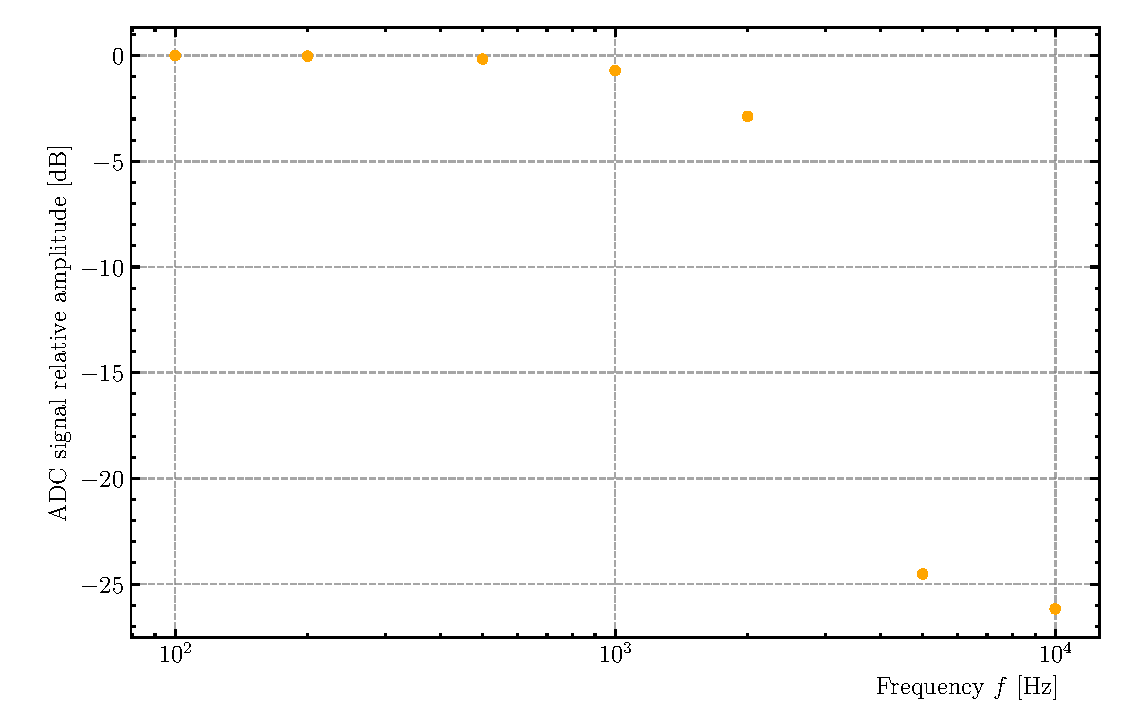
\includegraphics[width=\textwidth]{bode}
	\caption{Plot di Bode per l'ampiezza del segnale ricostruito dall'ADC per
	frequenze tra $\SI{100}{\Hz}$ e $\SI{10}{k\Hz}$ con segnale sinusoidale in
	ingresso di ampiezza fissata a $v\ped{in} = 2.5 \; \si{\V}$. Ad
	una frequenza di circa $\SI{2}{k\Hz}$ il grafico presenta un ginocchio in
	cui l'ampiezza è diminuita rispetto a centro banda di $-3$ dB.
	\label{fig: bode}}
\end{figure}
Da cui si vede di nuovo come l'uscita del circuito ha una risposta in frequenza
simile a quella di un integratore, come quello presente in \verb+U1+.

Come regola generale infatti ci aspettiamo che per riuscire a ricostruire
fedelmente il segnale in ingresso la frequenza di campionamento debba essere
almeno $f\ped{clk} \geq 20 f\ped{max}$ dove $f\ped{max}$ è la frequenza
massima dell'onda in ingresso.

\subsection{Stima del fattore di calibrazione del convertitore}
Per ottenere una legge di conversione tra i conteggi in uscita dall'ADC e
la d.d.p in Volt al suo ingresso abbiamo ricostruito alla stessa maniera dei
segnali di tensione nota e costante, in modo da esplorare il range di valori
ammessi per il nostro circuito. Per prima cosa ricaviamo il conteggio di zero
che corrisponde alla lettura in uscita dall'ADC con ingresso collegato a massa,
dunque effettuiamo un fit lineare per ricavare il fattore di scala per
convertire da Volt a conteggi dell'ADC.

Riportiamo in \cref{fig: cal} e di seguito i risultati del fit lineare
\begin{align*}
\mathrm{intercetta} &= 0.536 \pm 0.002 \; [\text{ADC counts}] \;\;\;
\mathrm{pendenza} = 0.155 \pm 0.007 \; [\si{counts/\V}] \\
\mathrm{correlazione} &= -0.97 \;\;\; \chi^2 = 0.1 \;\;\; \text{d.o.f.} = 10
\end{align*}

\begin{figure}[htbp]
    \centering
	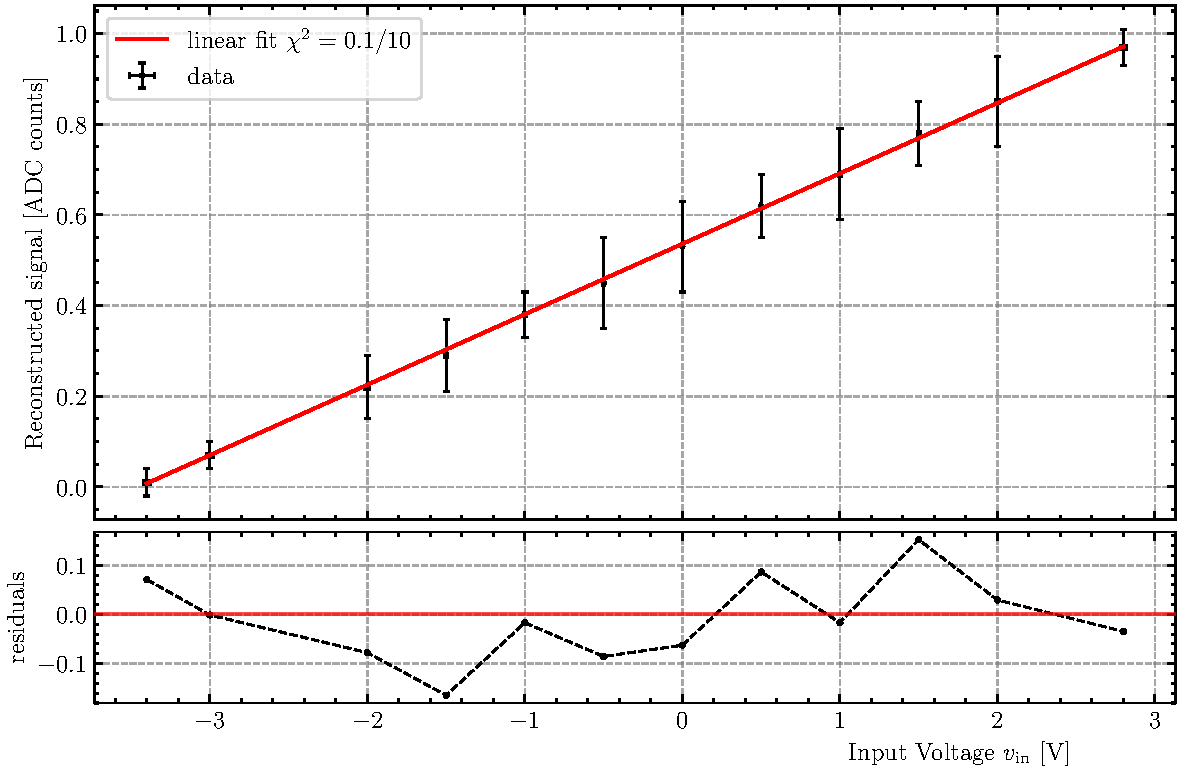
\includegraphics[width=\textwidth]{cal}
    \caption{Grafico con retta di best-fit e residui della lettura dell'ADC
    al variare della tensione in ingresso per la calibrazione dell'ADC
    \label{fig: cal}}
\end{figure}

Si utilizza anche un secondo metodo per la calibrazione inversa del circuito;
per cui ad un conteggio ricostruito dall'ADC $Y \in [0, 1]$ corrisponde una
misura in Volt $X = (Y - O) \cdot C$.

Dopo avere eseguito il fit dell'onda ricostruita, si divide l'ampiezza
dell'onda in ingresso misurata tramite oscilloscopio, per il valore
dell'ampiezza ricavato dal fit, da cui otteniamo
\begin{align*}
C &= 6.39 \pm 0.06 \; \si{\V/counts} \\
O &= 471 \times 10^{-3} \pm 2 \times 10^{-4} \; \text{ADC counts}
\end{align*}

\subsection{Misura del signal/noise ratio (SNR)}
Assumendo che il valore RMS del rumore del nostro circuito corrisponda al
valore RMS dei residui del fit alla sinusoide effettuato in \cref{sbs: freq},
si è stimato il rapporto segnale/rumore in potenza tramite la formula
\begin{equation}\label{eq: SNR}
\text{SNR} = \frac{A_{pp}^2/8}{\sigma^2\ped{noise}} =
\frac{A^2/2}{\text{Var}(\text{residuals})} = 380
\end{equation}
in cui $A_{pp}$ è l'ampiezza massima (picco-picco) e $\sigma\ped{noise}$ indica
il valore rms del rumore.

Dunque abbiamo ricavato il numero di bit effettivi del convertitore studiato
tramite la formula
\begin{equation}\label{eq: effbit}
n\ped{bits} = \frac{20\log_{10}{\text{SNR}} - 1.76 \; \si{dB}}
{6.02 \; \si{dB}} = 8.3
\end{equation}

\subsection*{Nota sul metodo di fit}
Per determinare i parametri ottimali e le rispettive covarianze si \`e
implementato in \verb+Python+ un algoritmo di fit basato sui minimi quadrati
mediante la funzione \emph{curve\_fit} della libreria \texttt{SciPy}.

%=======================
\section*{Conclusioni e commenti finali}
Si è riusciti a costruire e studiare il comportamento di un convertitore
analogico-digitale Sigma-Delta facendo uso di tre amplificatori
operazionali (TL081) e un D-FF (74LS74).

In particolare si è riusciti a descrivere e verificare sperimentalmente il
corretto funzionamento del circuito e a caratterizzarne la risposta in uscita
sia nel dominio dei tempi che delle frequenze al variare dei parametri del
segnale analogico inviato al suo ingresso.

%=======================
\section*{Dichiarazione}
I firmatari di questa relazione dichiarano che il contenuto della relazione \`e
originale, con misure effettuate dai membri del gruppo, e che tutti i firmatari
hanno contribuito alla elaborazione della relazione stessa.

\end{document}